\documentclass[12pt,a4paper]{report}

%% ================= PACKAGES =================
\usepackage[margin=1in]{geometry}
\usepackage{newtxtext,newtxmath}
\usepackage{setspace}
\usepackage{ragged2e}
\usepackage{tabularx}
\usepackage{array}
\usepackage{graphicx}
\usepackage{caption}
\usepackage{float}
\usepackage{titlesec}
\usepackage{fancyhdr}
\usepackage{etoolbox}
\usepackage{xcolor}
\usepackage{listings}
\usepackage{xurl}
\usepackage{hyperref}
\usepackage{pdfpages}

\lstset{
    basicstyle=\ttfamily\small,
    breaklines=true,
    breakatwhitespace=false,
    columns=fullflexible,
    keepspaces=true,
    frame=single,
    numbers=left,
    numberstyle=\tiny,
    tabsize=4,
    showstringspaces=false
}

\hypersetup{
    colorlinks=true,
    linkcolor=black,
    citecolor=black,
    urlcolor=blue,
    pageanchor=true
}

%% =====================================================
%% FILL THIS — update before compiling
%% =====================================================

\newcommand{\ProjectTitle}{Your Project Title Goes Here}
\newcommand{\HeaderTitle}{Short Project Title}
\newcommand{\AcademicYear}{2025--2026}
\newcommand{\DepartmentName}{Department of CSE (Data Science)}

\newcommand{\StudentOne}{Student One Full Name}
\newcommand{\USNOne}{1DSXXCDXXX}
\newcommand{\StudentTwo}{Student Two Full Name}
\newcommand{\USNTwo}{1DSXXCDXXX}
\newcommand{\StudentThree}{Student Three Full Name}
\newcommand{\USNThree}{1DSXXCDXXX}
\newcommand{\StudentFour}{Student Four Full Name}
\newcommand{\USNFour}{1DSXXCDXXX}

\newcommand{\GuideName}{Dr. Guide Name}
\newcommand{\GuideDesignation}{Associate Professor, Dept. of CSE (Data Science), DSCE}
\newcommand{\ProjectCoordinator}{Dr. Coordinator Name}
\newcommand{\HODName}{Dr. HOD Full Name}
\newcommand{\PrincipalName}{Dr. Principal Name}

%% =====================================================
%% PAGE SETTINGS
%% =====================================================

\renewcommand{\arraystretch}{1.2}
\setlength{\headheight}{16pt}
\onehalfspacing
\setlength{\parindent}{0pt}
\setlength{\parskip}{6pt}
\raggedbottom
\AtBeginEnvironment{titlepage}{\setstretch{1.0}}

\titleformat{\chapter}[display]
  {\centering\bfseries\fontsize{16}{20}\selectfont}
  {\chaptername\ \thechapter}{10pt}{\centering}

\titleformat{\section}
  {\bfseries\fontsize{14}{16}\selectfont}{\thesection}{1em}{}

\fancypagestyle{mainstyle}{
  \fancyhf{}
  \lhead{\small\textbf{\HeaderTitle}}
  \rhead{\small\textbf{\AcademicYear}}
  \lfoot{\small \DepartmentName}
  \rfoot{\small Page \thepage}
  \renewcommand{\headrulewidth}{0.4pt}
  \renewcommand{\footrulewidth}{0.4pt}
}

\fancypagestyle{plain}{
  \fancyhf{}
  \lhead{\small\textbf{\HeaderTitle}}
  \rhead{\small\textbf{\AcademicYear}}
  \lfoot{\small \DepartmentName}
  \rfoot{\small Page \thepage}
  \renewcommand{\headrulewidth}{0.4pt}
  \renewcommand{\footrulewidth}{0.4pt}
}

%% =====================================================
\begin{document}
\hypersetup{pageanchor=false}
\pagestyle{empty}

%% =====================================================
%% TITLE PAGE
%% =====================================================

\begin{titlepage}
\centering
\vspace*{0.2cm}

{\Large \bfseries Visvesvaraya Technological University \\[0.2em]}
{\large \bfseries Belgaum, Karnataka- 590014 \\[0.6em]}


\includegraphics[width=2.8cm]{images/VTULogo.png}

\vspace{0.5em}

{\large Third Year \\[0.15em]}
{\large \bfseries A Mini-Project Report \\[0.3em]}
{\large On \\[0.3em]}
{\large \bfseries ``\ProjectTitle'' \\[0.8em]}

{\normalsize Submitted in the partial fulfilment of the requirements for the award of the Degree of \\[0.45em]}

{\large \bfseries BACHELOR OF ENGINEERING \\[0.15em]}
{\normalsize In \\[0.15em]}
{\large \bfseries COMPUTER SCIENCE AND ENGINEERING \\[0.15em]}
{\large \bfseries (DATA SCIENCE) \\[0.8em]}

{\normalsize Submitted by \\[0.35em]}
{\normalsize \bfseries
  \StudentOne\ (\USNOne) \\
  \StudentTwo\ (\USNTwo) \\
  \StudentThree\ (\USNThree) \\
  \StudentFour\ (\USNFour) \\[0.8em]
}

{\normalsize Under the Guidance of \\[0.3em]}
{\normalsize \bfseries \GuideName \\[0.15em]}
{\small \GuideDesignation \\[0.8em]}


\includegraphics[width=2.2cm]{images/DSCELogo.png}

\vspace{0.5em}

{\normalsize \AcademicYear \\[0.25em]}
{\normalsize \bfseries DEPARTMENT OF CSE (DATA SCIENCE) \\[0.15em]}
{\normalsize \bfseries DAYANANDA SAGAR COLLEGE OF ENGINEERING \\[0.3em]}
{\small SHAVIGE MALLESHWARA HILLS, KUMARASWAMY LAYOUT, BANGALORE-78}

\vfill
\end{titlepage}

%% =====================================================
%% CERTIFICATE
%% =====================================================

\clearpage
\begin{center}

{\Large \bfseries DAYANANDA SAGAR COLLEGE OF ENGINEERING \\[0.3em]}
{\normalsize Shavige Malleshwara Hills, Kumaraswamy Layout \\ Bangalore-560078 \\[0.7em]}
{\Large \bfseries Department of CSE (DATA SCIENCE) \\[0.5em]}


\includegraphics[width=2.2cm]{images/DSCELogo.png} \\[0.8em]

{\large \AcademicYear \\[0.9em]}
{\LARGE \bfseries Certificate \\[1.2em]}

\begin{spacing}{1.25}
\justify
\begin{center}
\parbox{0.95\textwidth}{
This is to certify that the Mini Project Work entitled
\textbf{``\ProjectTitle''}
is a bonafide work carried out by
\textbf{\StudentOne\ (\USNOne), \StudentTwo\ (\USNTwo),
\StudentThree\ (\USNThree) and \StudentFour\ (\USNFour)},
in partial fulfilment for the VI semester of Bachelor of Engineering in
CSE (Data Science) of the Visvesvaraya Technological University, Belgaum
during the year \AcademicYear.
The Project report has been approved as it satisfies the academic requirements
prescribed for the Bachelor of Engineering degree.
}
\end{center}
\end{spacing}

\vspace{2.5cm}

\begin{tabularx}{\textwidth}{
  >{\centering\arraybackslash}X
  >{\centering\arraybackslash}X
  >{\centering\arraybackslash}X
}
Signature of Project Coordinator & Signature of Guide & Signature of HOD \\[0.2cm]
[\ProjectCoordinator] & [\GuideName] & [\HODName]
\end{tabularx}

\vspace{1cm}

\begin{tabularx}{\textwidth}{p{8cm} X}
\hspace{1cm}\textbf{Name of the Examiners} & \textbf{Signature with Date} \\[0.4cm]
1. & \\[0.9cm]
2. &
\end{tabularx}

\end{center}

%% =====================================================
%% ACKNOWLEDGEMENT
%% =====================================================

\clearpage
\pagenumbering{roman}
\setcounter{page}{1}
\pagestyle{mainstyle}

\chapter*{ACKNOWLEDGEMENT}
\addcontentsline{toc}{chapter}{ACKNOWLEDGEMENT}

\setlength{\parindent}{1.5em}
\setlength{\parskip}{0.8em}
\setstretch{1.5}

First and foremost, we thank the Almighty for the blessings and guidance throughout this project.

We express our sincere gratitude to our Principal, \PrincipalName, for providing all necessary facilities.

We thank our Head of Department, \HODName, for the constant motivation and support extended to us.

We extend our heartfelt thanks to our guide, \GuideName, for the valuable guidance and suggestions throughout the project.

We are grateful to all teaching and non-teaching staff of the Department of CSE (Data Science) for their direct and indirect support. We also thank our family and friends for their encouragement throughout.

\setlength{\parindent}{0pt}
\setlength{\parskip}{6pt}
\onehalfspacing

%% =====================================================
%% TABLE OF CONTENTS
%% =====================================================

\clearpage
\begingroup
\setstretch{1.0}
\setlength{\parskip}{0pt}
\pagestyle{mainstyle}
\thispagestyle{mainstyle}
\renewcommand{\contentsname}{CONTENTS}
\tableofcontents
\endgroup

\clearpage
\hypersetup{pageanchor=true}
\pagenumbering{arabic}
\setcounter{page}{1}
\pagestyle{mainstyle}

%% =====================================================
\chapter{Introduction}
%% Replace with your project introduction.
%% Cover: problem statement, motivation, limitations of existing work,
%% what you propose, and the structure of the report.

Lorem ipsum dolor sit amet, consectetur adipiscing elit. Sed do eiusmod tempor incididunt ut labore et dolore magna aliqua. Ut enim ad minim veniam, quis nostrud exercitation ullamco laboris nisi ut aliquip ex ea commodo consequat.

Duis aute irure dolor in reprehenderit in voluptate velit esse cillum dolore eu fugiat nulla pariatur. Excepteur sint occaecat cupidatat non proident, sunt in culpa qui officia deserunt mollit anim id est laborum.

Sed ut perspiciatis unde omnis iste natus error sit voluptatem accusantium doloremque laudantium, totam rem aperiam, eaque ipsa quae ab illo inventore veritatis et quasi architecto beatae vitae dicta sunt explicabo.

%% =====================================================
\chapter{Literature Survey}
%% One paragraph per paper reviewed.
%% Format: what they did, method/dataset, result, limitation.
%% Cite using \cite{key}. Add entries to references.bib.

Lorem ipsum dolor sit amet~\cite{ref1}, consectetur adipiscing elit. Sed do eiusmod tempor incididunt ut labore et dolore magna aliqua. Ut enim ad minim veniam, quis nostrud exercitation ullamco laboris nisi ut aliquip ex ea commodo consequat.

Duis aute irure dolor~\cite{ref2} in reprehenderit in voluptate velit esse cillum dolore eu fugiat nulla pariatur. Excepteur sint occaecat cupidatat non proident, sunt in culpa qui officia deserunt mollit anim id est laborum.

Lorem ipsum dolor sit amet~\cite{ref3}, consectetur adipiscing elit. Sed ut perspiciatis unde omnis iste natus error sit voluptatem accusantium doloremque laudantium.

Nemo enim ipsam voluptatem~\cite{ref4} quia voluptas sit aspernatur aut odit aut fugit, sed quia consequuntur magni dolores eos qui ratione voluptatem sequi nesciunt.

At vero eos et accusamus~\cite{ref5} et iusto odio dignissimos ducimus qui blanditiis praesentium voluptatum deleniti atque corrupti quos dolores et quas molestias excepturi sint.

Lorem ipsum dolor sit amet, consectetur adipiscing elit. Sed do eiusmod tempor incididunt ut labore et dolore magna aliqua, quis nostrud exercitation ullamco laboris nisi ut aliquip ex ea commodo consequat.

%% =====================================================
\chapter{Research Gap Identified}
%% Each bullet = one gap from the literature.
%% Each gap should justify a design choice in your system.

From the literature survey, the following research gaps are identified:

\begin{itemize}
    \item Lorem ipsum dolor sit amet, consectetur adipiscing elit, sed do eiusmod tempor incididunt ut labore et dolore magna aliqua.

    \item Ut enim ad minim veniam, quis nostrud exercitation ullamco laboris nisi ut aliquip ex ea commodo consequat duis aute irure dolor.

    \item Excepteur sint occaecat cupidatat non proident, sunt in culpa qui officia deserunt mollit anim id est laborum sed ut perspiciatis.

    \item Nemo enim ipsam voluptatem quia voluptas sit aspernatur aut odit aut fugit, sed quia consequuntur magni dolores eos qui ratione.

    \item At vero eos et accusamus et iusto odio dignissimos ducimus qui blanditiis praesentium voluptatum deleniti atque corrupti quos dolores.

    \item Therefore, there is a need to develop a system that addresses the above limitations and demonstrates practical applicability in a real-world context.
\end{itemize}

%% =====================================================
\chapter{Architectures}
%% Replace each images/placeholder.png with your actual diagram file.
%% All diagrams can go in images/Diagrams/ for organisation.

\section{High Level Architecture}

The high level architecture of the proposed system is shown in Figure~\ref{fig:high_level_arch}.

\begin{figure}[H]
    \centering
    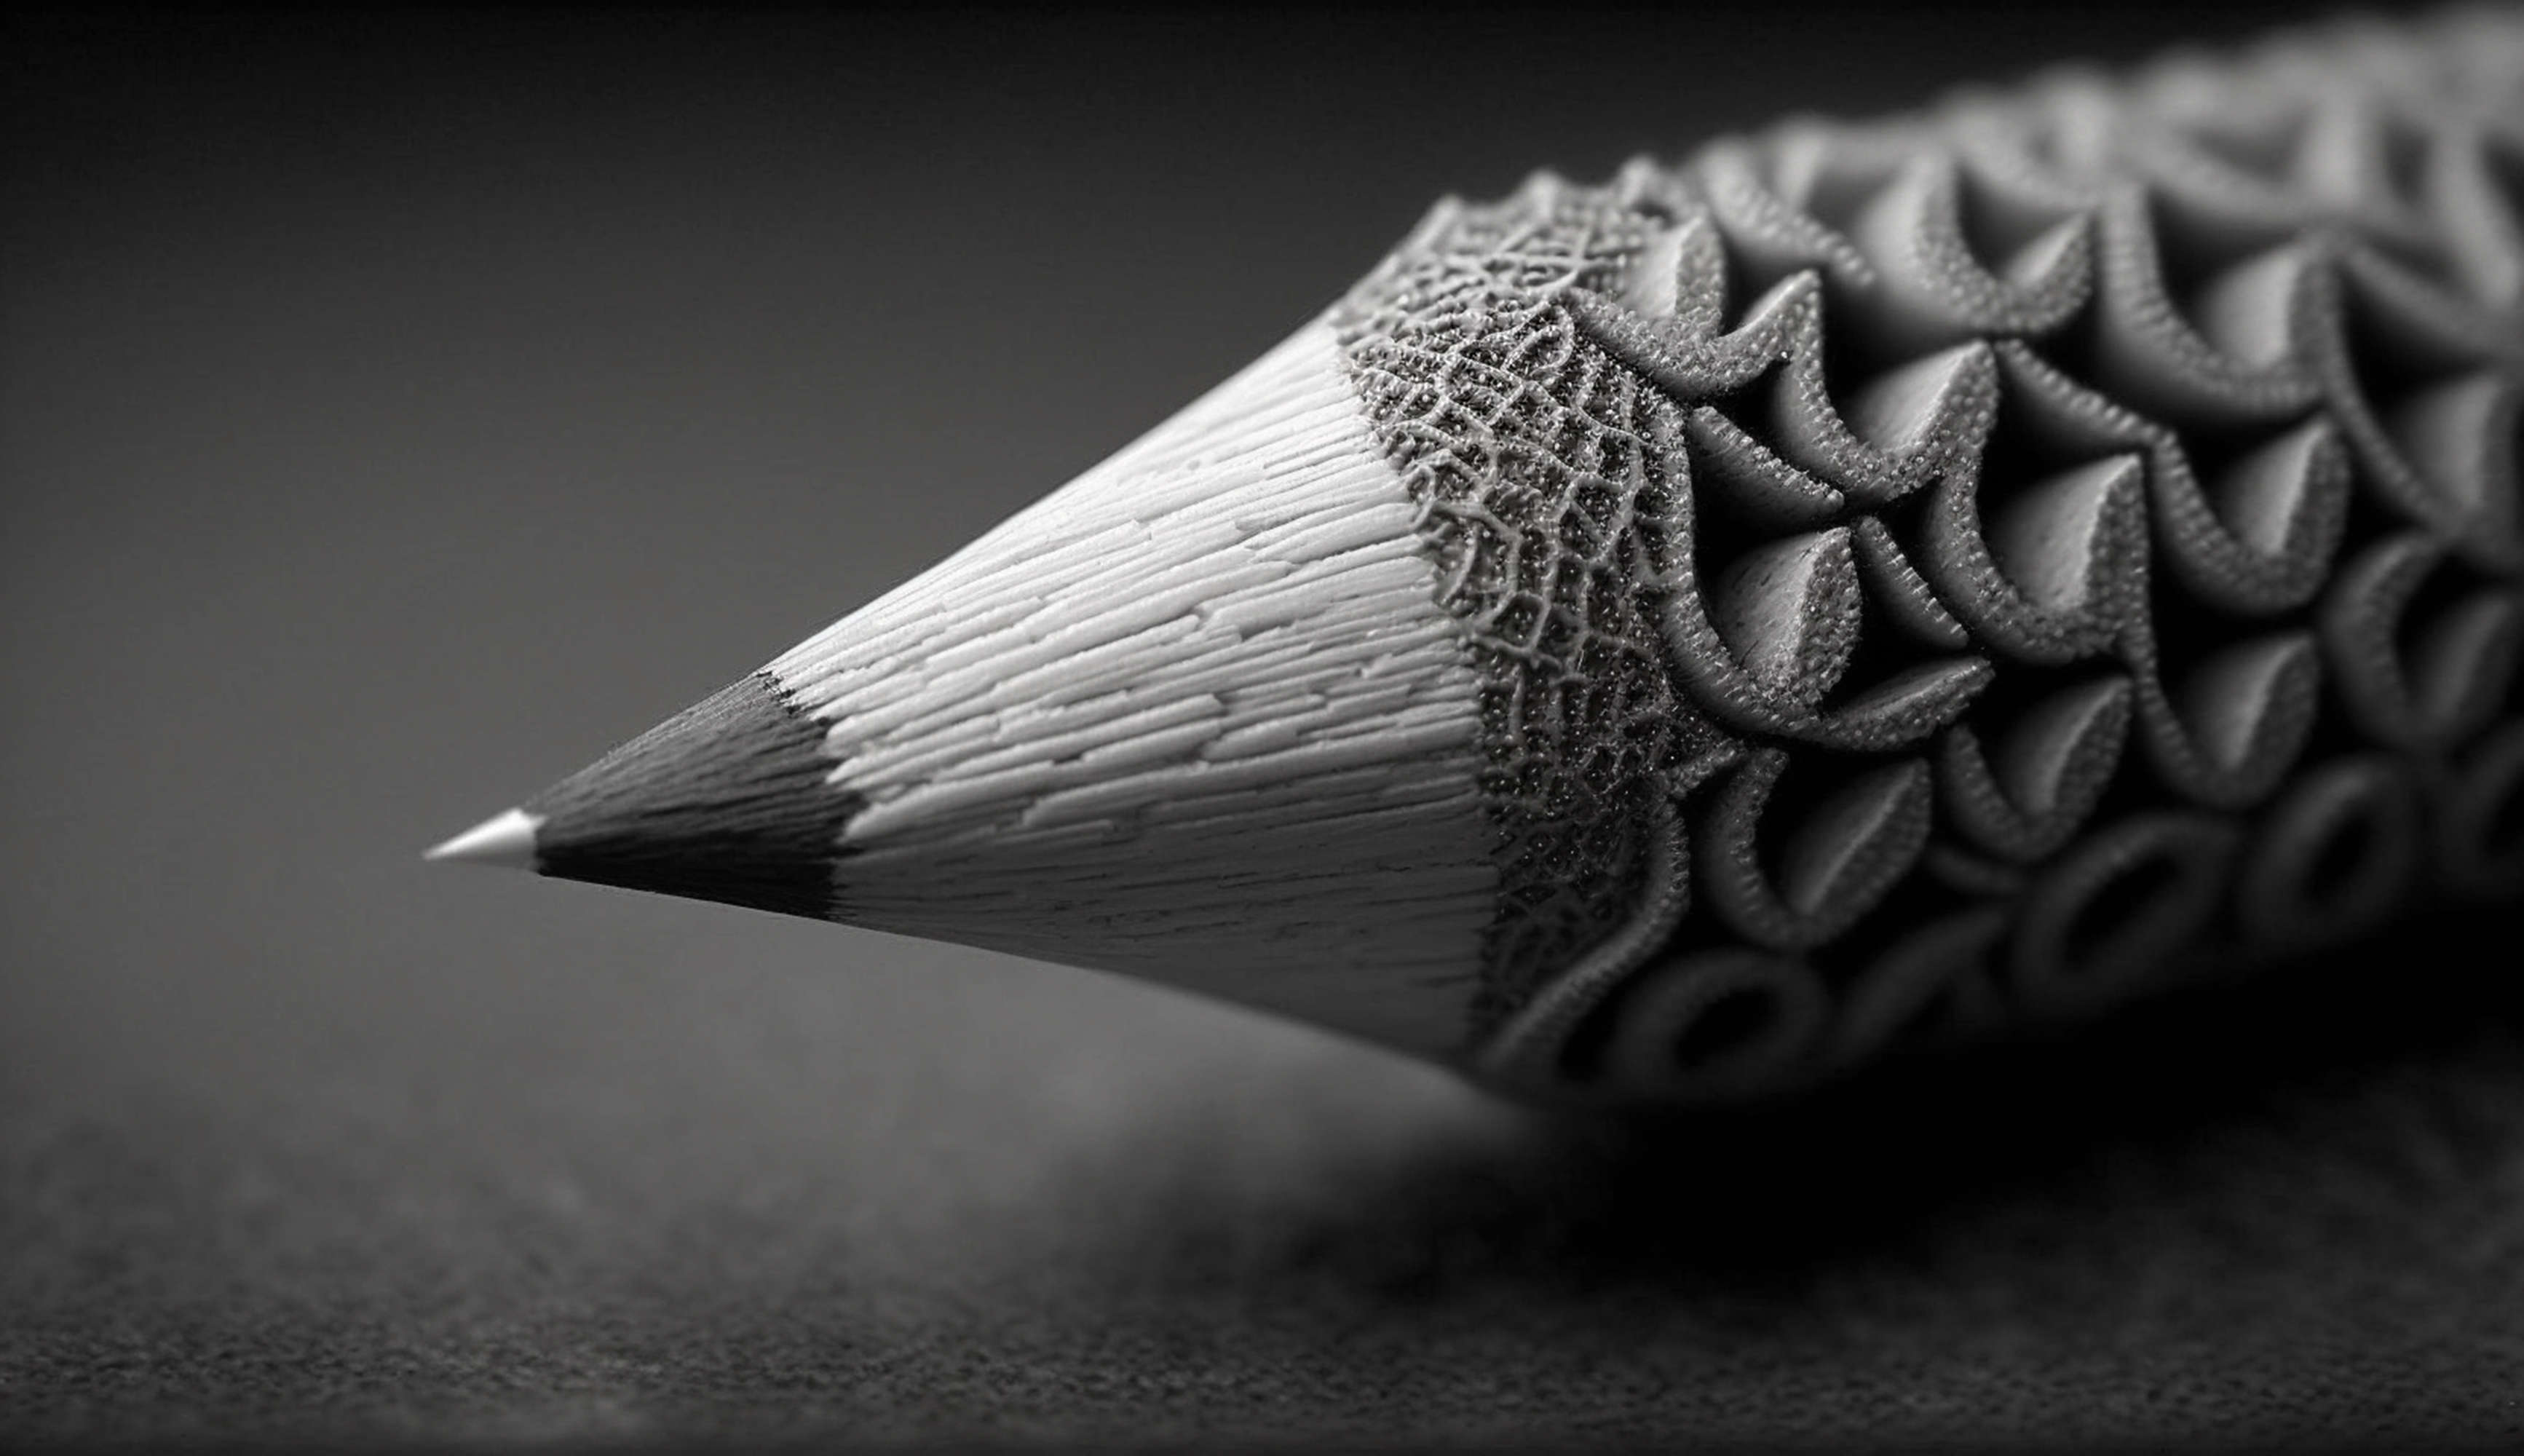
\includegraphics[width=0.65\textwidth]{images/placeholder.png}
    \caption{High Level Architecture of the Proposed System}
    \label{fig:high_level_arch}
\end{figure}

\section{Use Case Diagram}

The use case diagram shown in Figure~\ref{fig:use_case} represents the interaction between the user and the proposed system.

\begin{figure}[H]
    \centering
    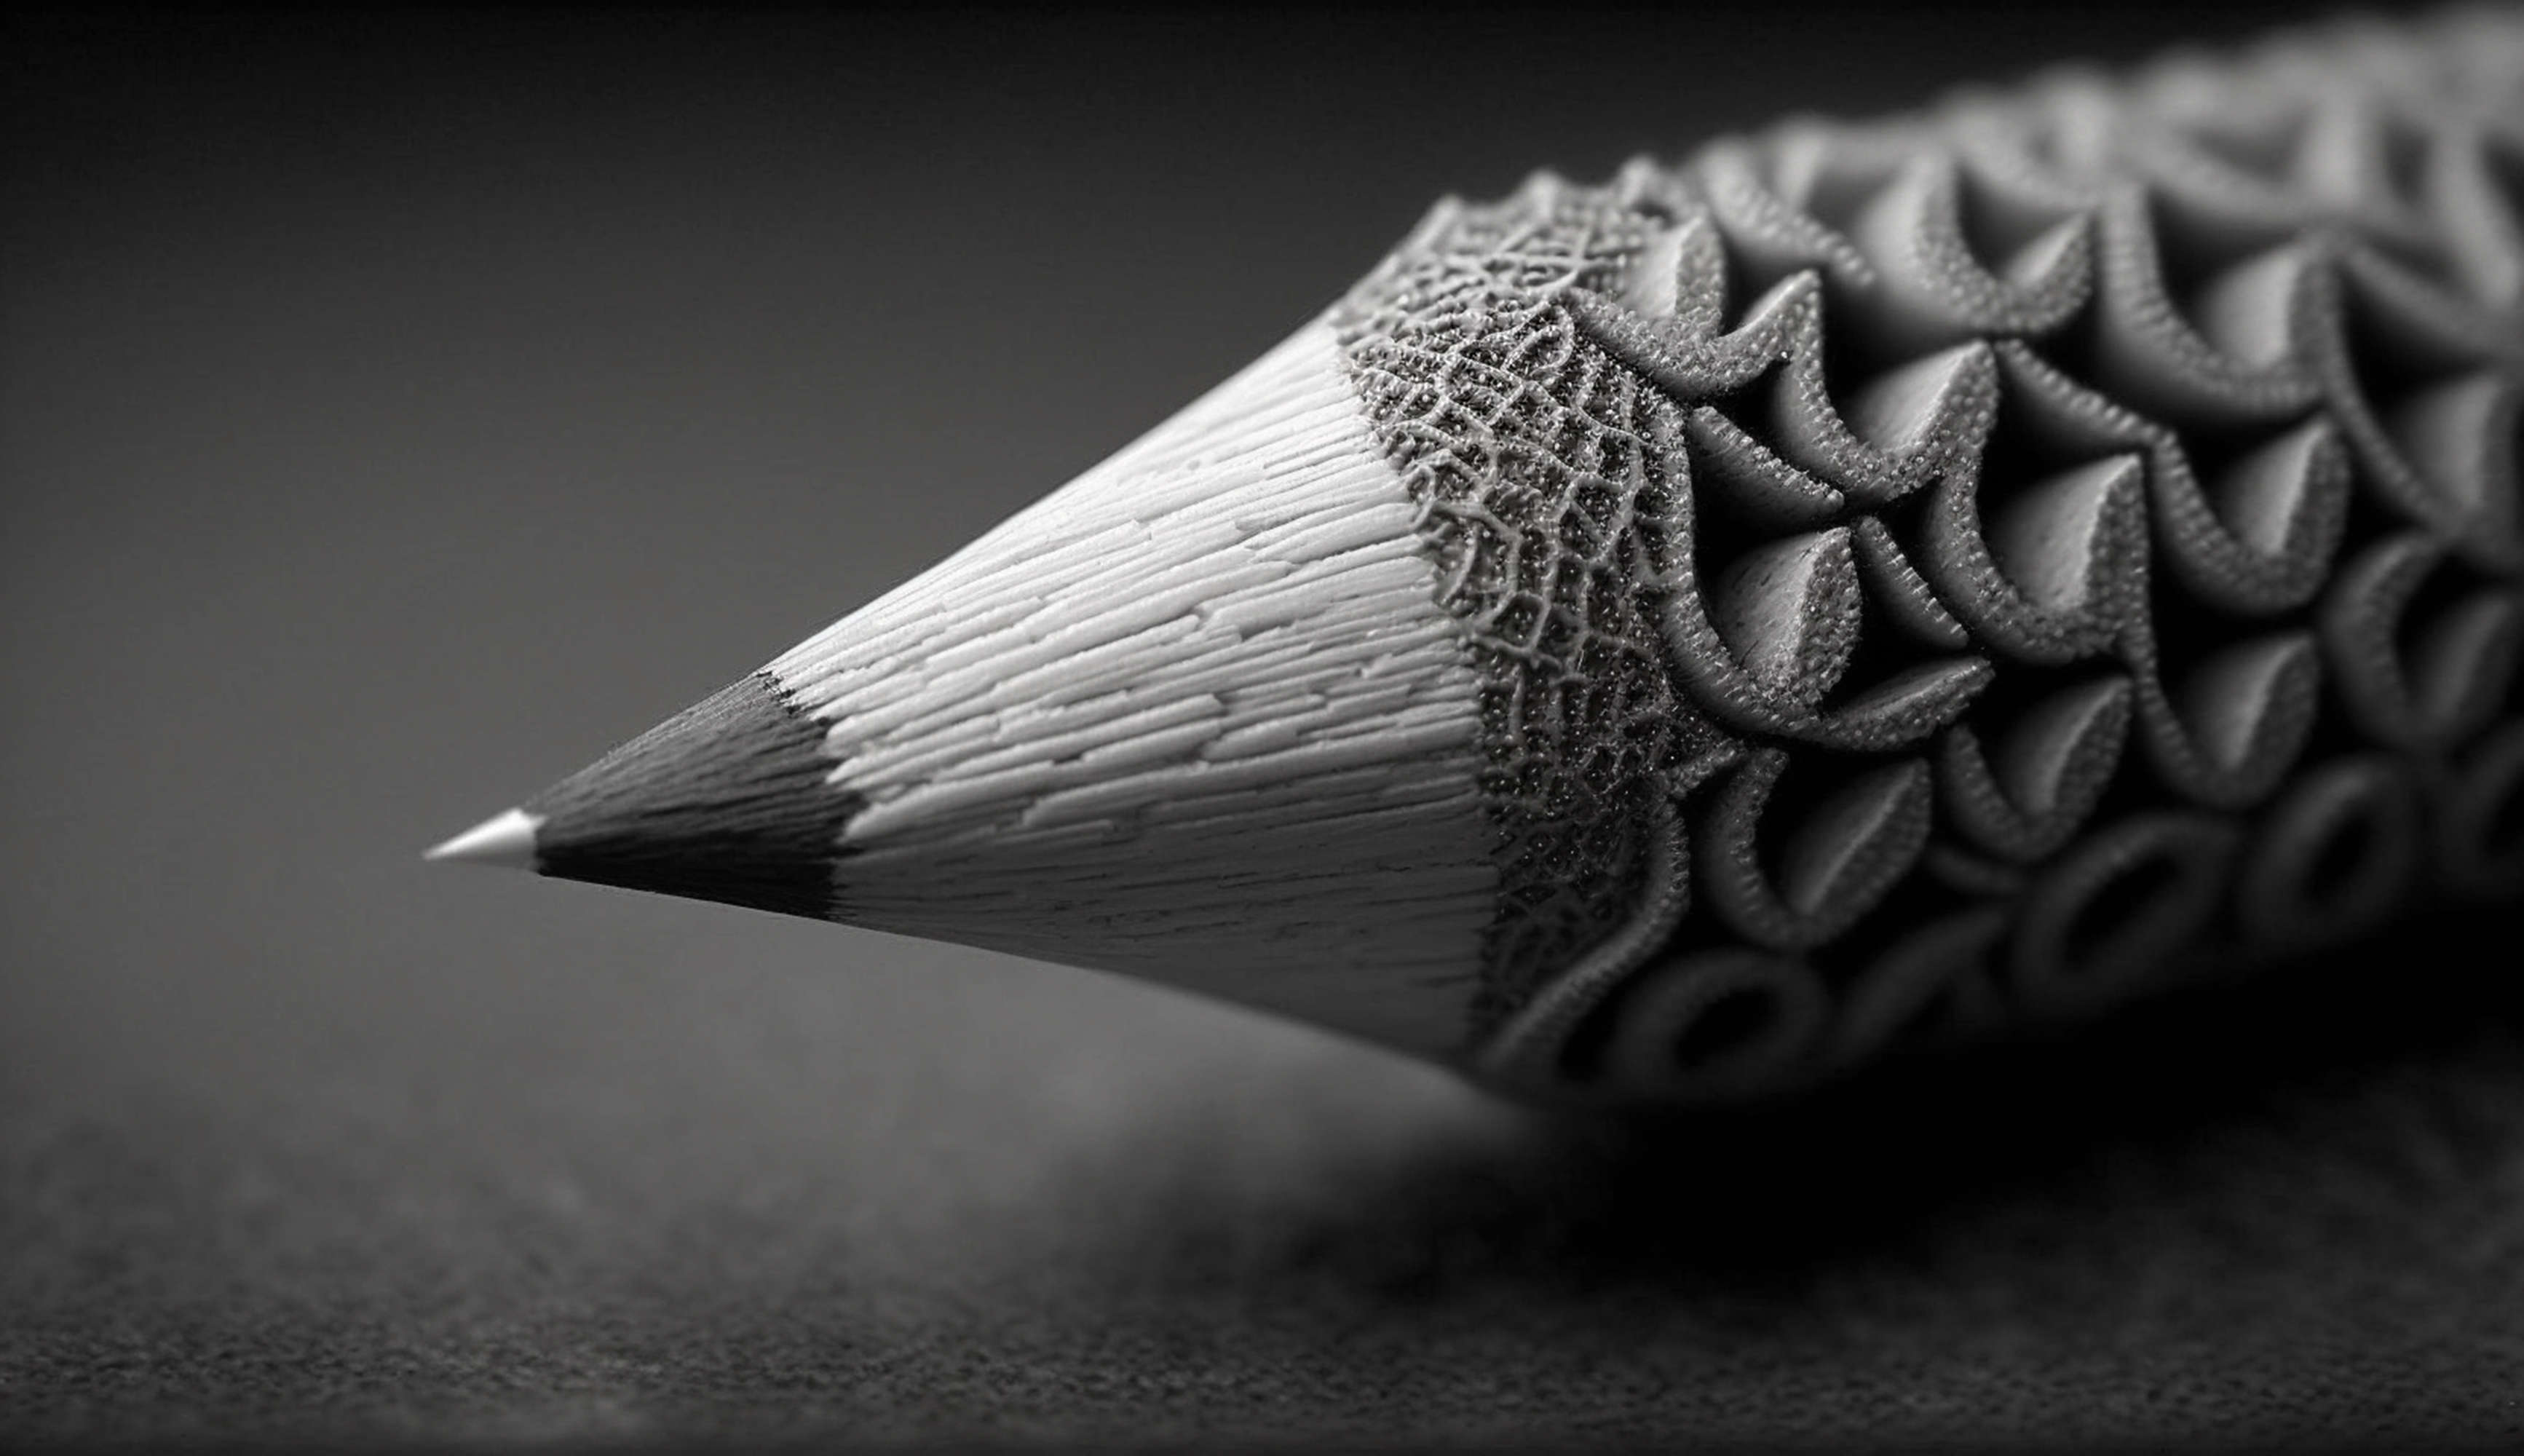
\includegraphics[width=0.55\textwidth]{images/placeholder.png}
    \caption{Use Case Diagram of the Proposed System}
    \label{fig:use_case}
\end{figure}

\section{Data Flow Diagram}

\subsection{Level 0 DFD}

\begin{figure}[H]
    \centering
    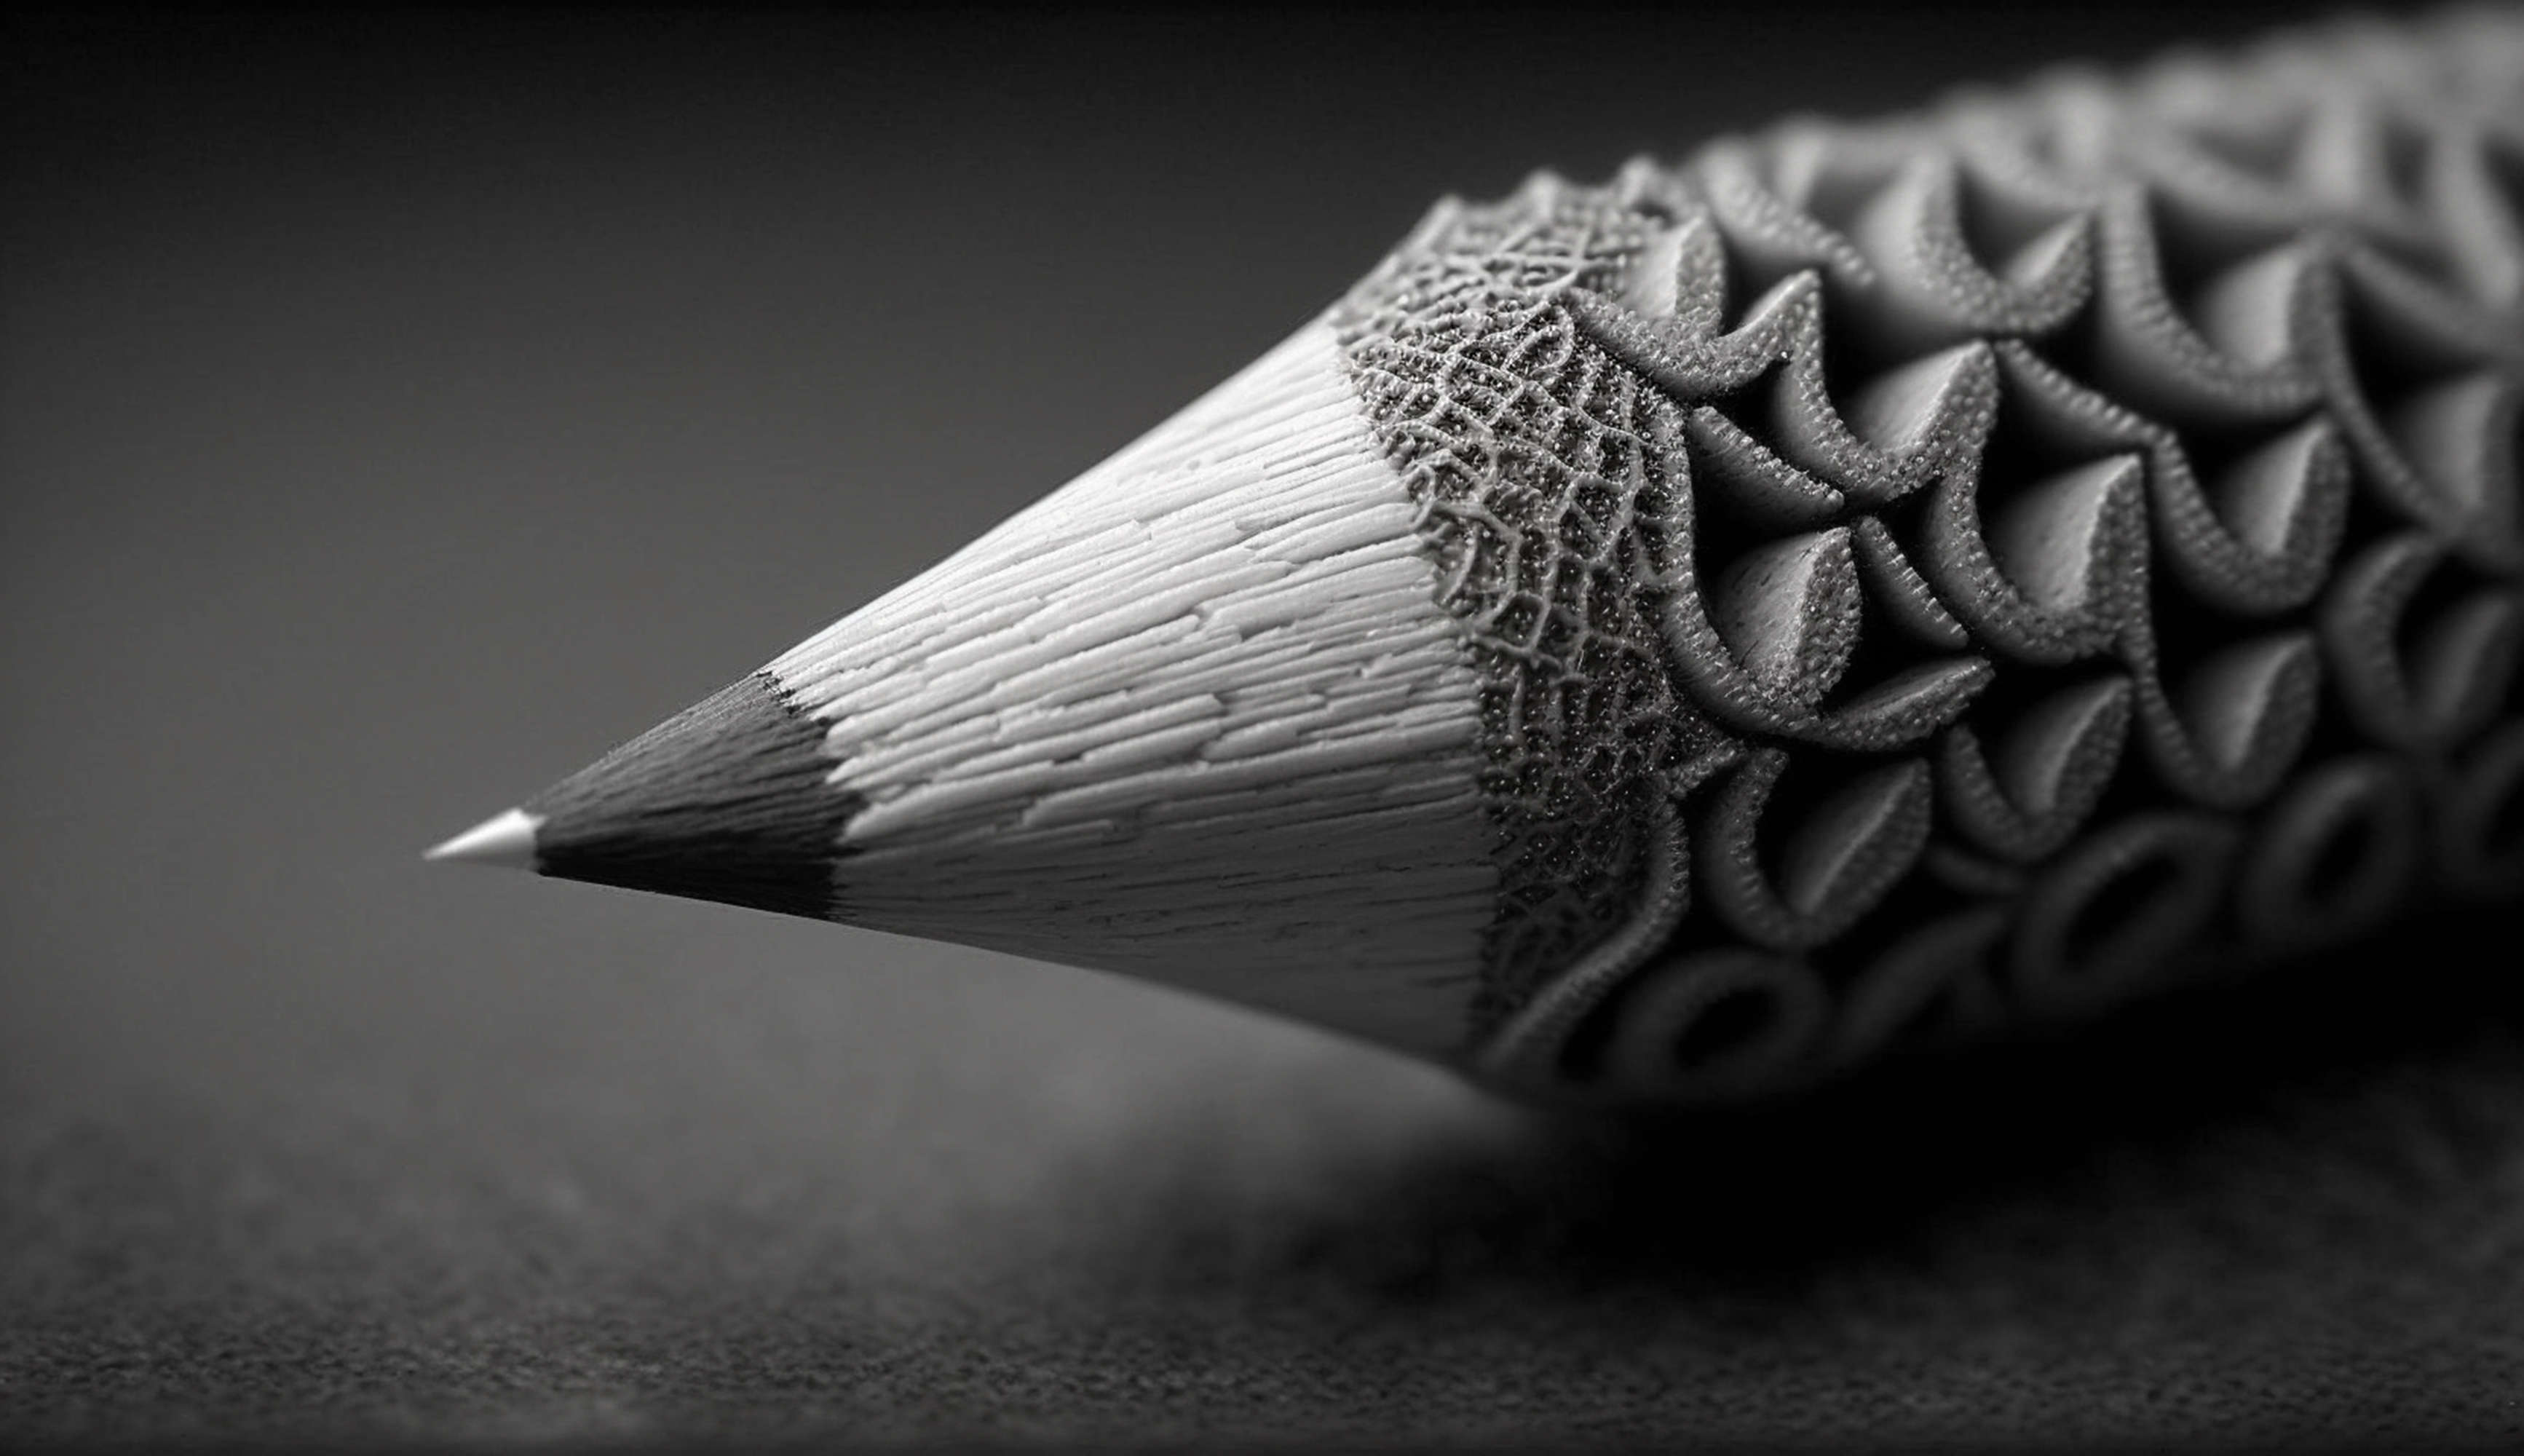
\includegraphics[width=0.7\textwidth]{images/placeholder.png}
    \caption{Level 0 Data Flow Diagram}
    \label{fig:dfd0}
\end{figure}

\subsection{Level 1 DFD}

\begin{figure}[H]
    \centering
    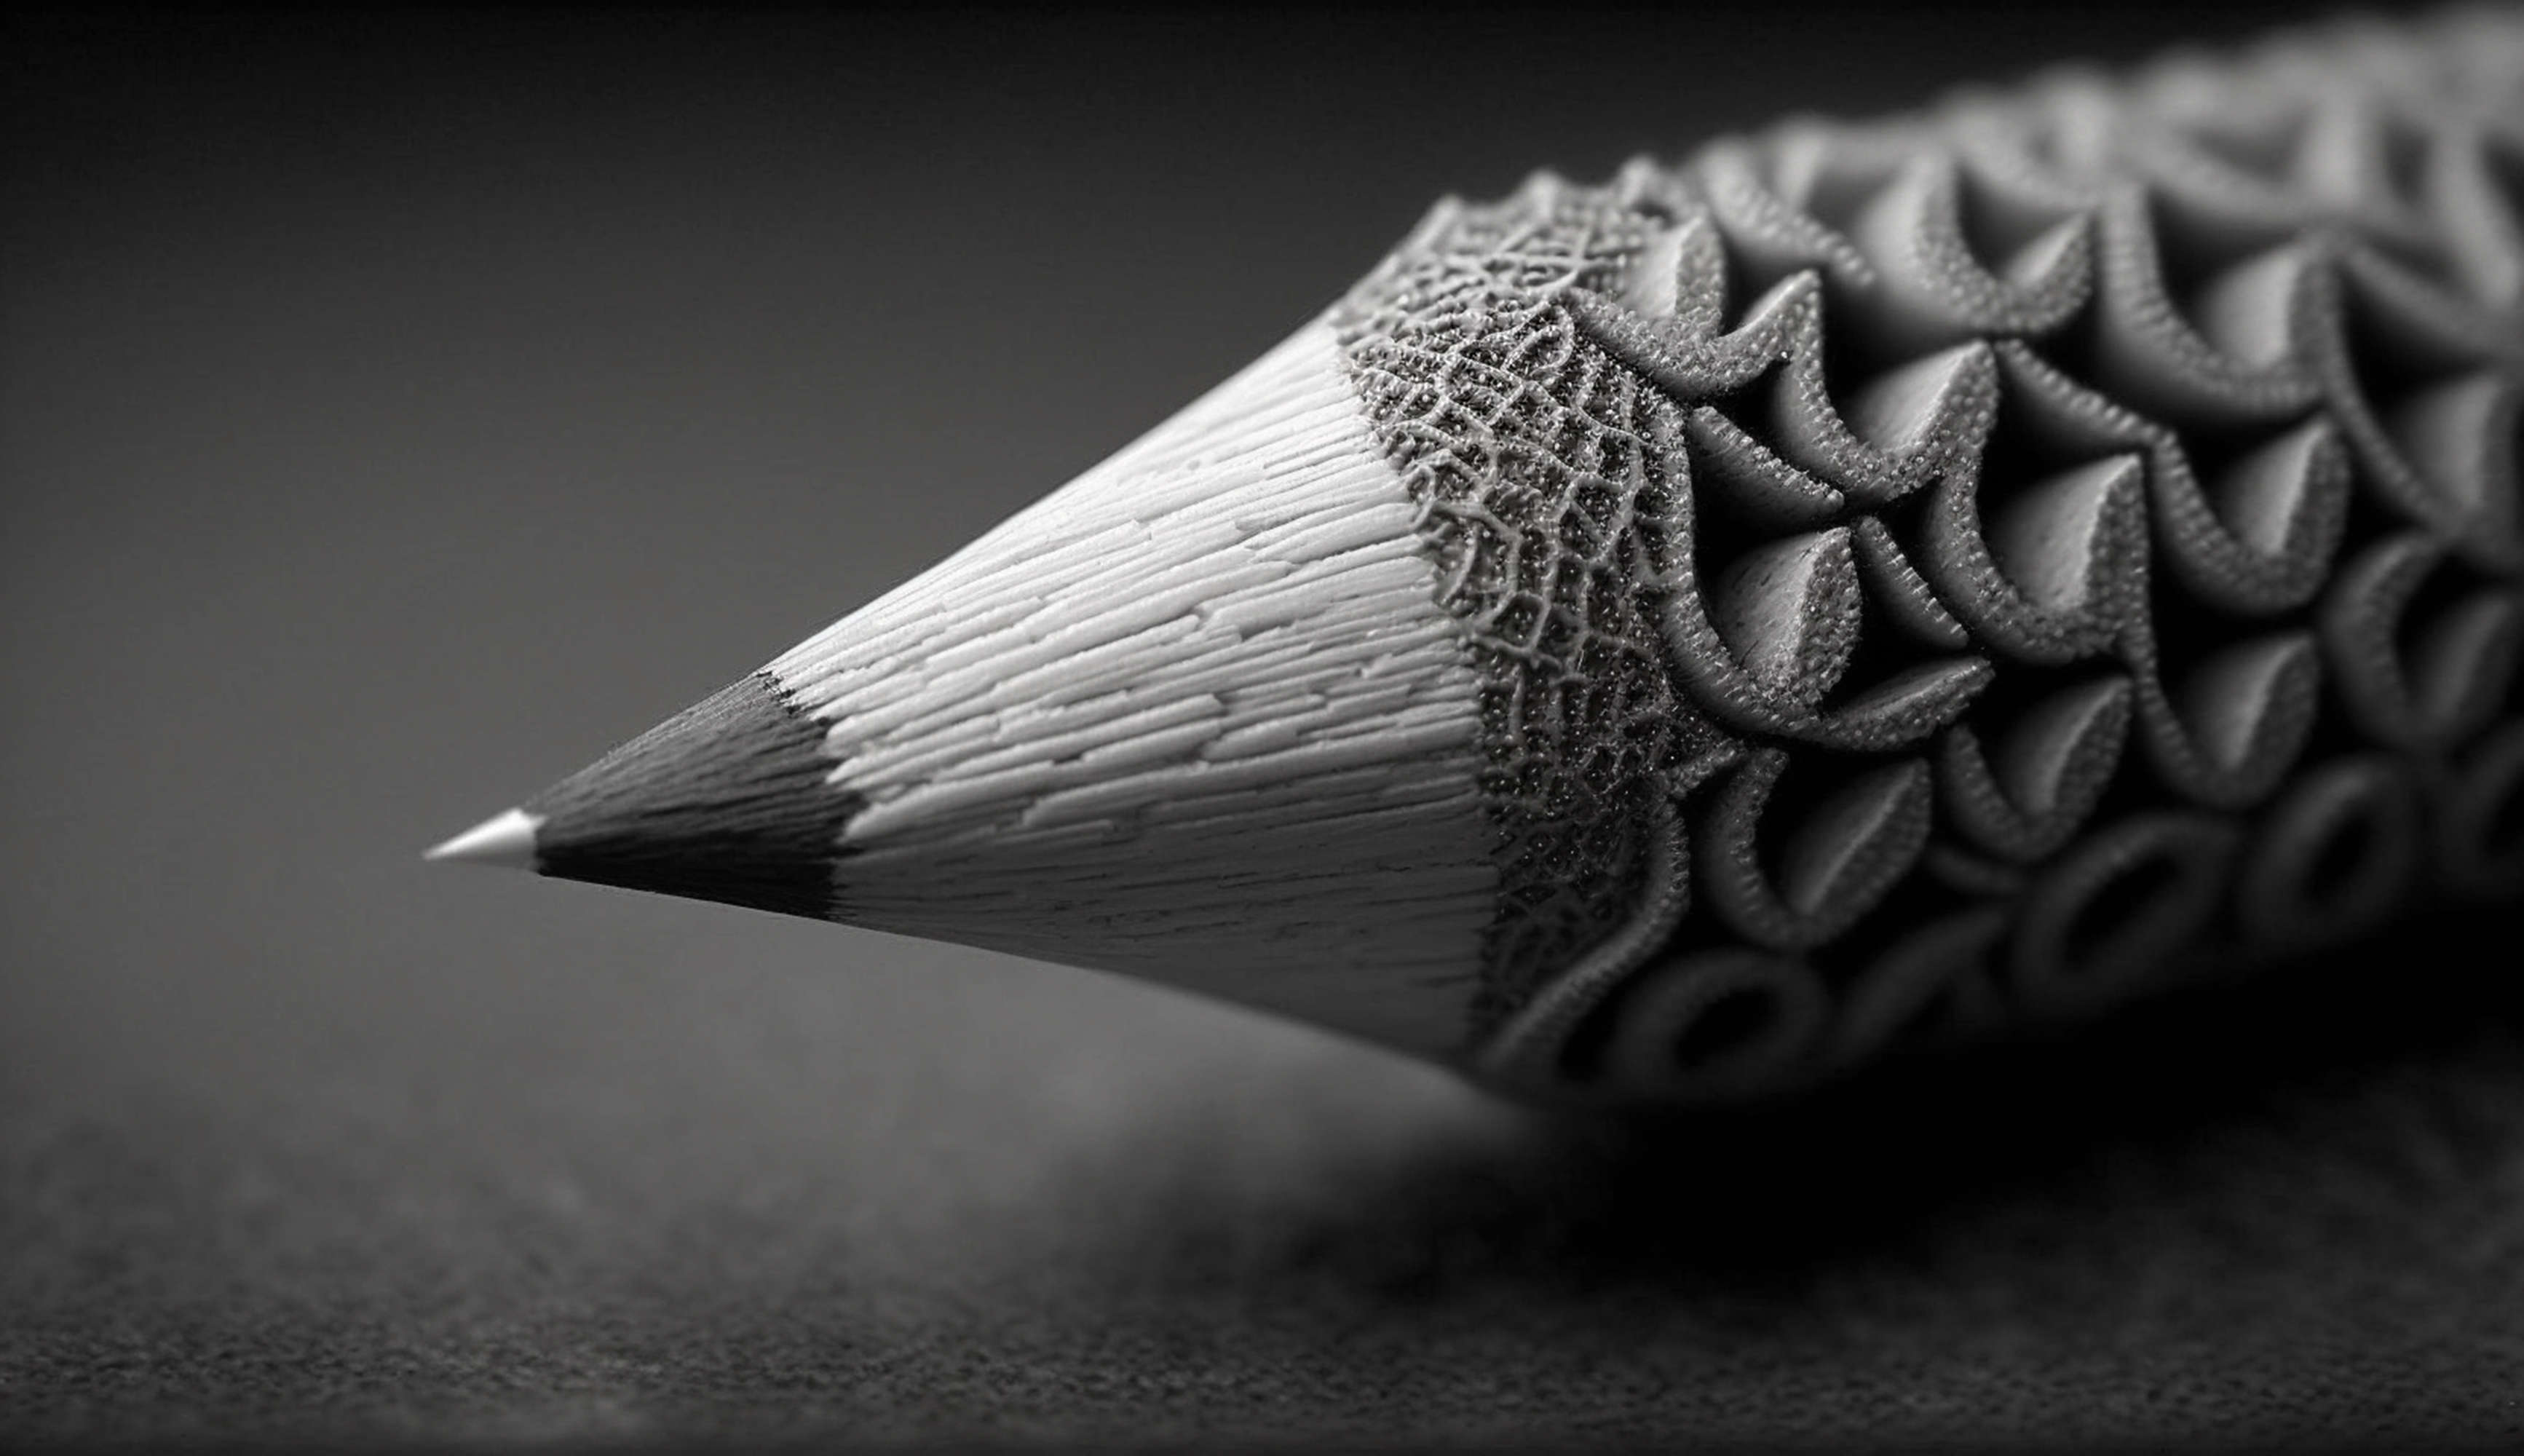
\includegraphics[width=0.9\textwidth]{images/placeholder.png}
    \caption{Level 1 Data Flow Diagram}
    \label{fig:dfd1}
\end{figure}

\section{Detailed System Architecture}

\subsection{Input Processing Layer}

\begin{figure}[H]
    \centering
    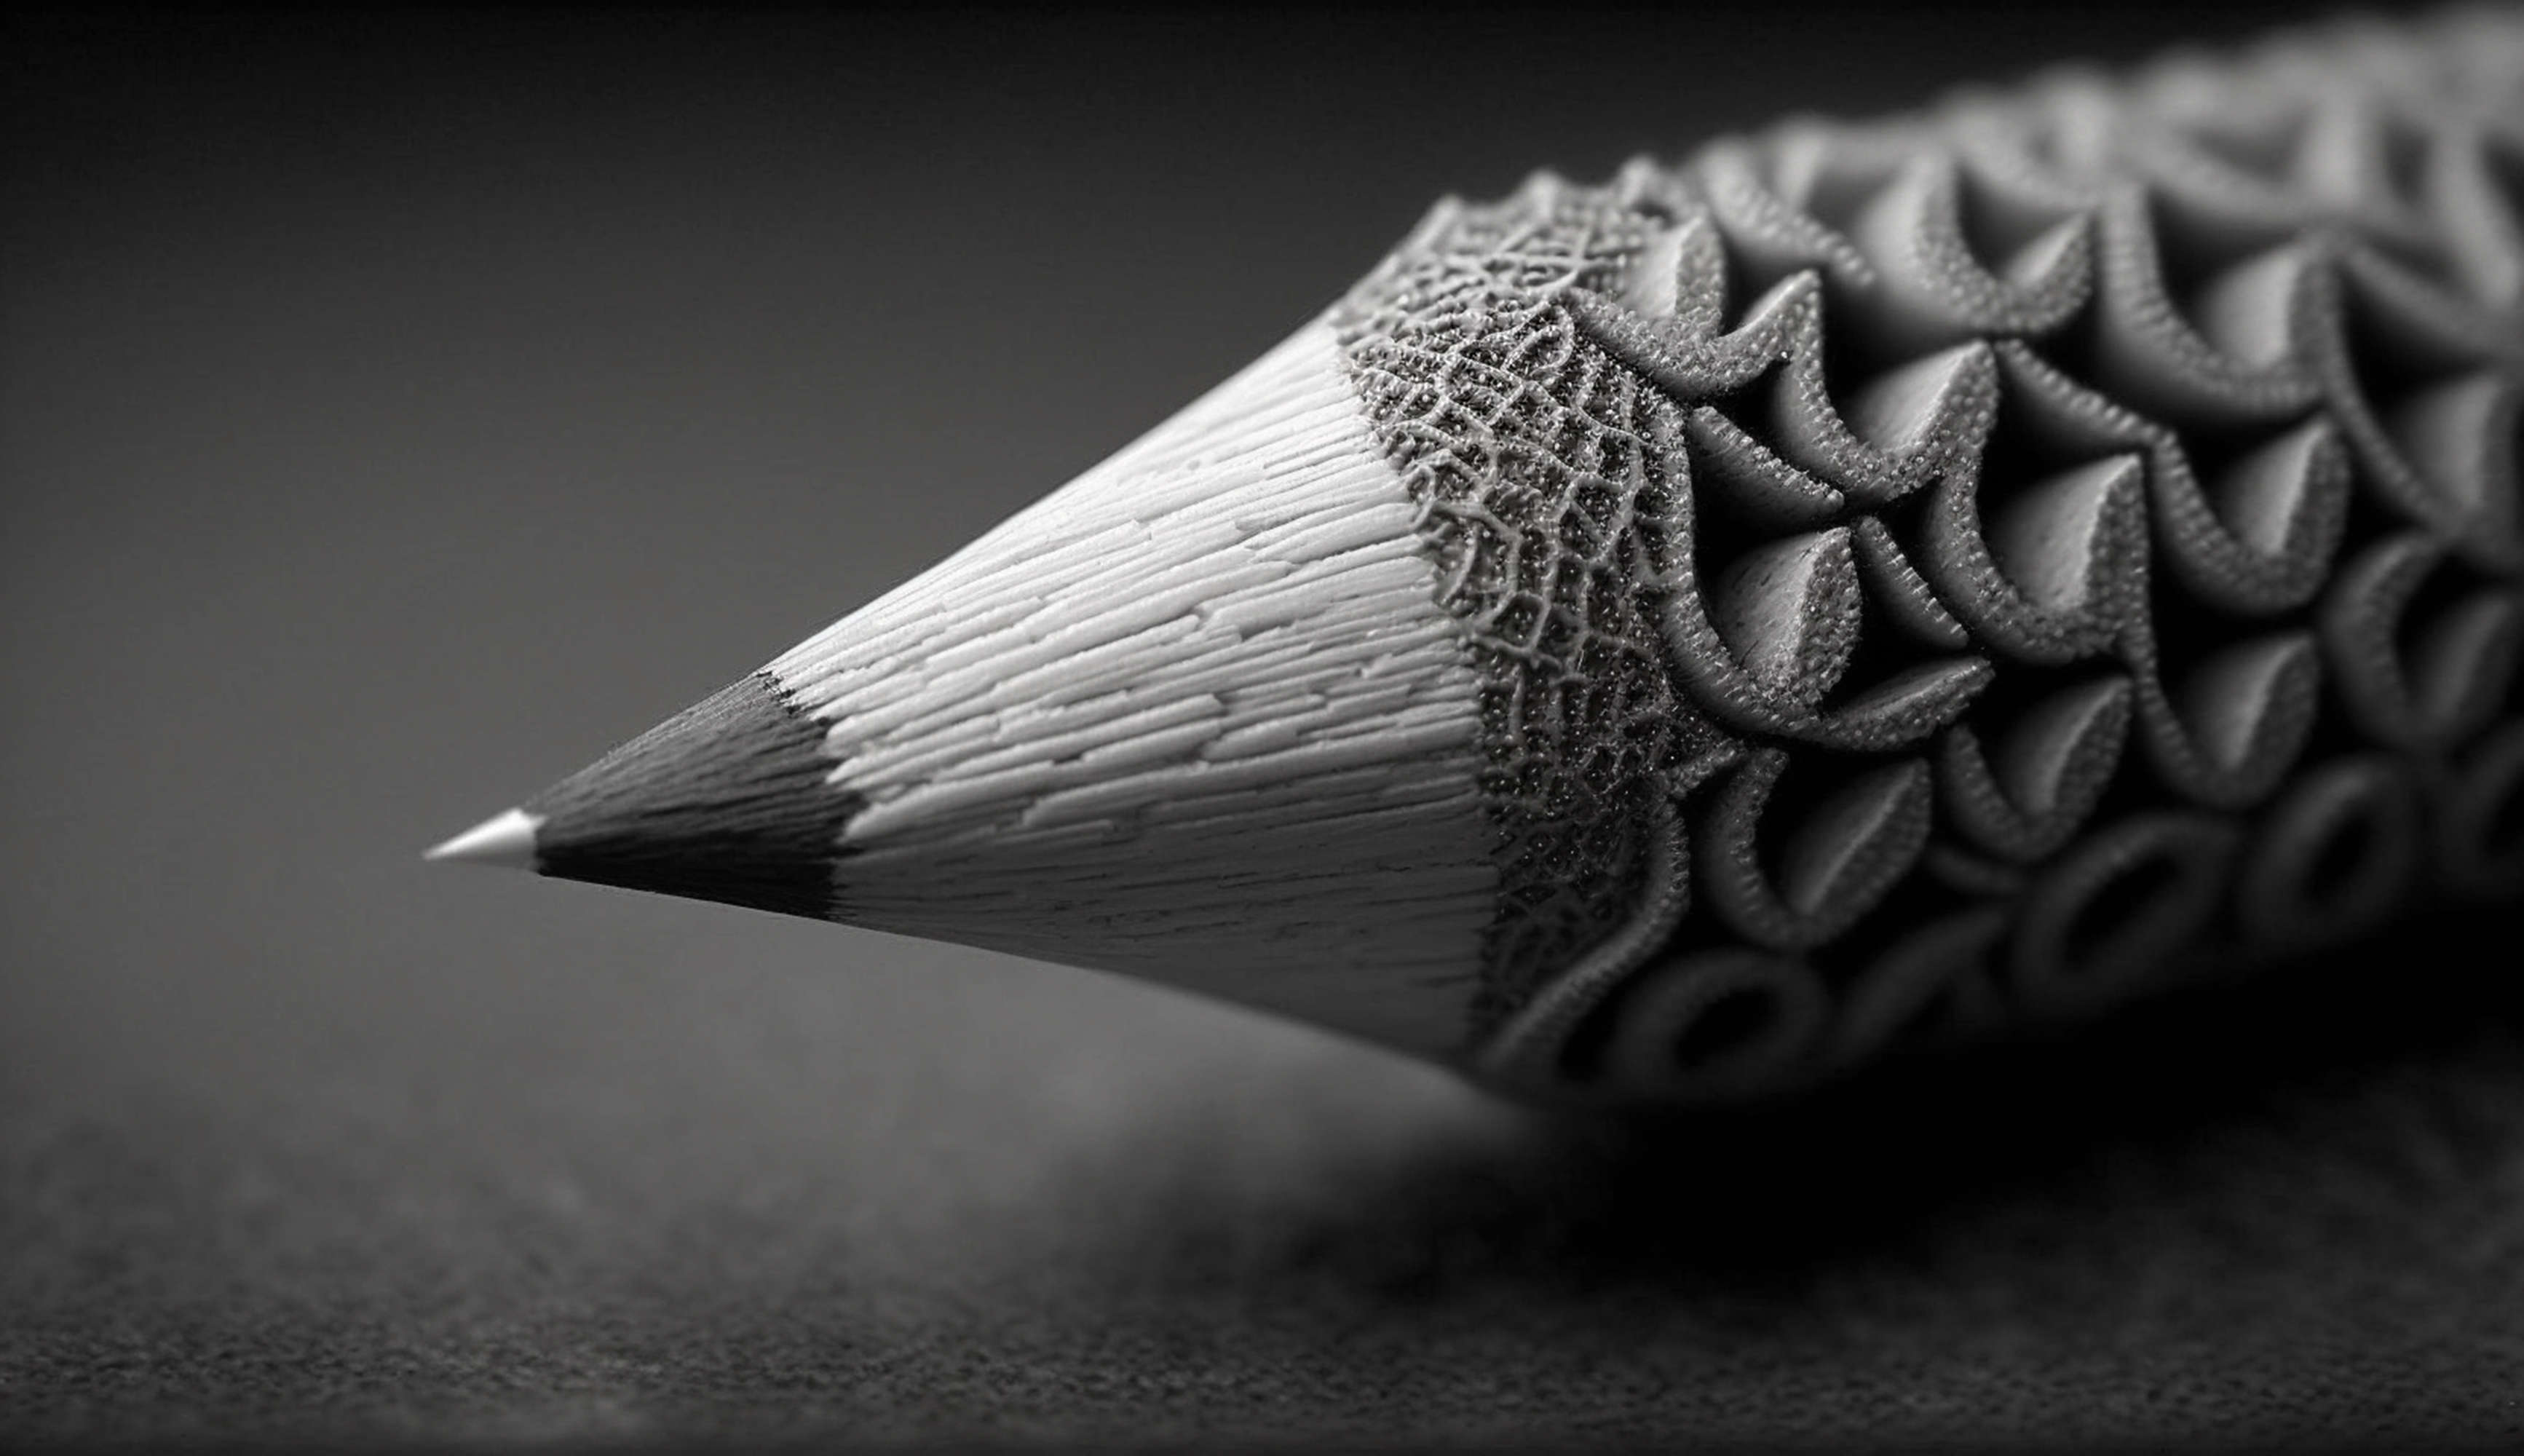
\includegraphics[width=0.9\textwidth]{images/placeholder.png}
    \caption{Detailed Architecture -- Input Processing Layer}
    \label{fig:arch1}
\end{figure}

\subsection{Model and Core Processing Layer}

\begin{figure}[H]
    \centering
    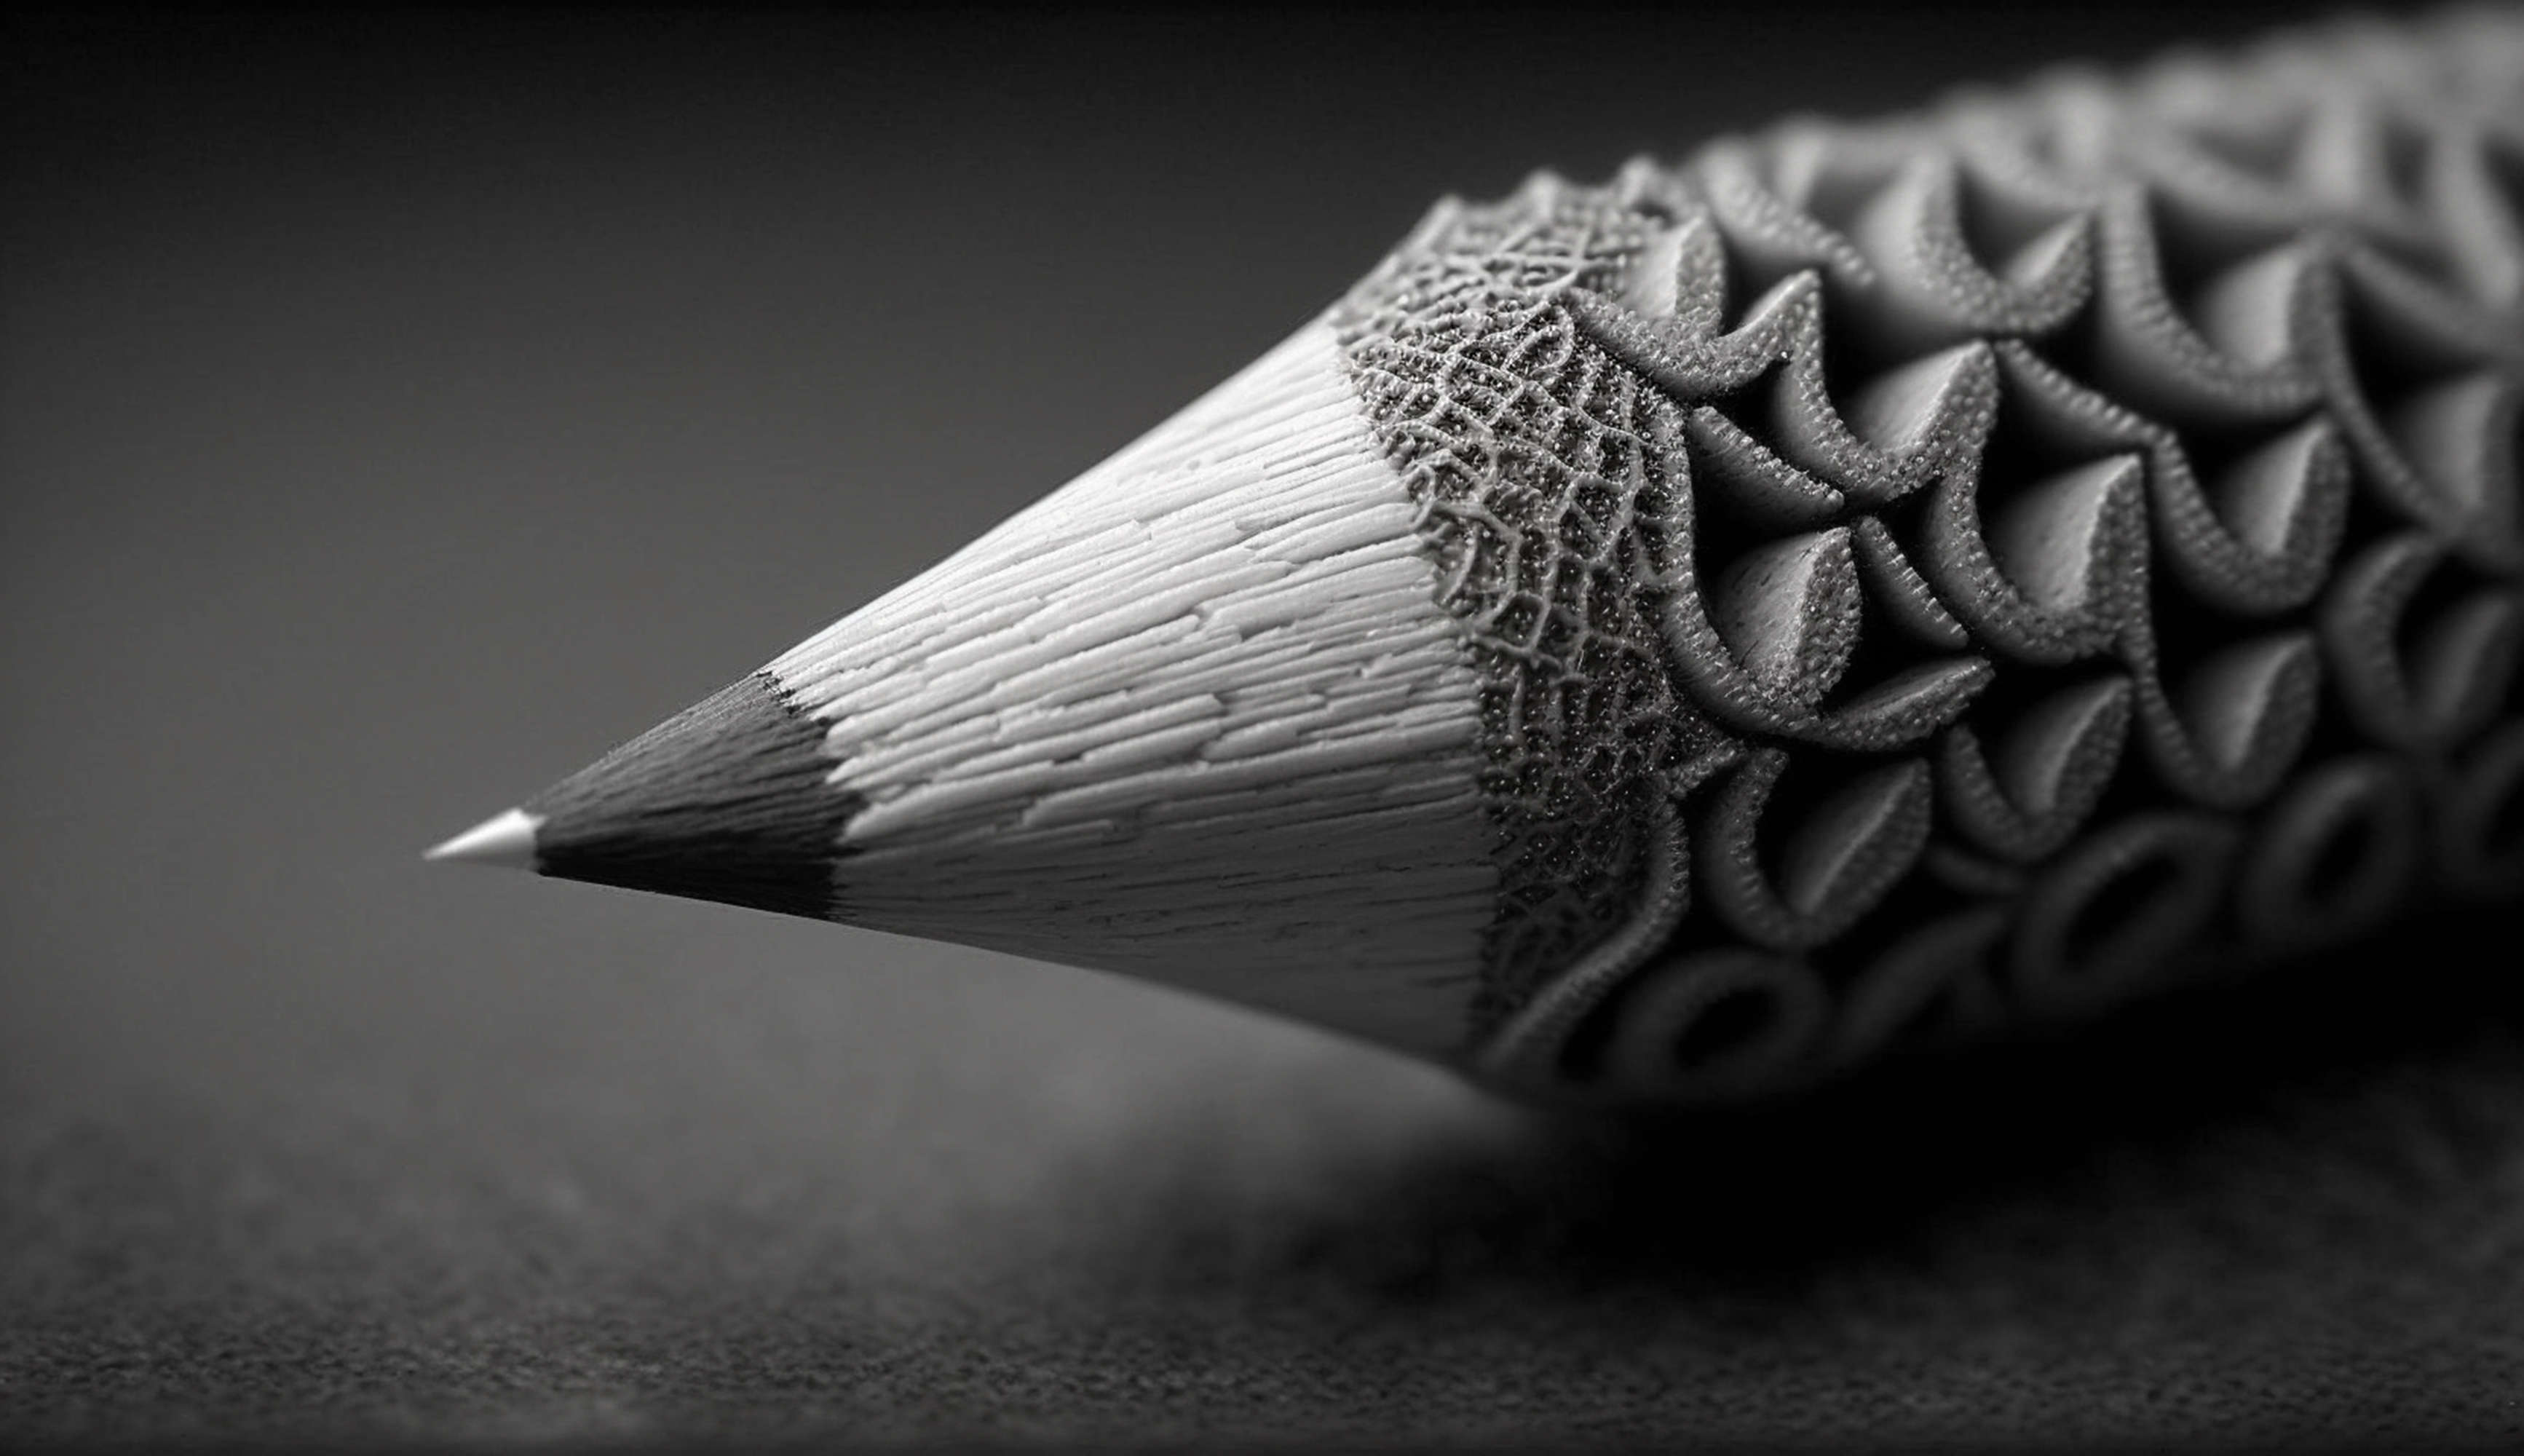
\includegraphics[width=0.9\textwidth]{images/placeholder.png}
    \caption{Detailed Architecture -- Model and Core Processing Layer}
    \label{fig:arch2}
\end{figure}

\subsection{Output and Recommendation Layer}

\begin{figure}[H]
    \centering
    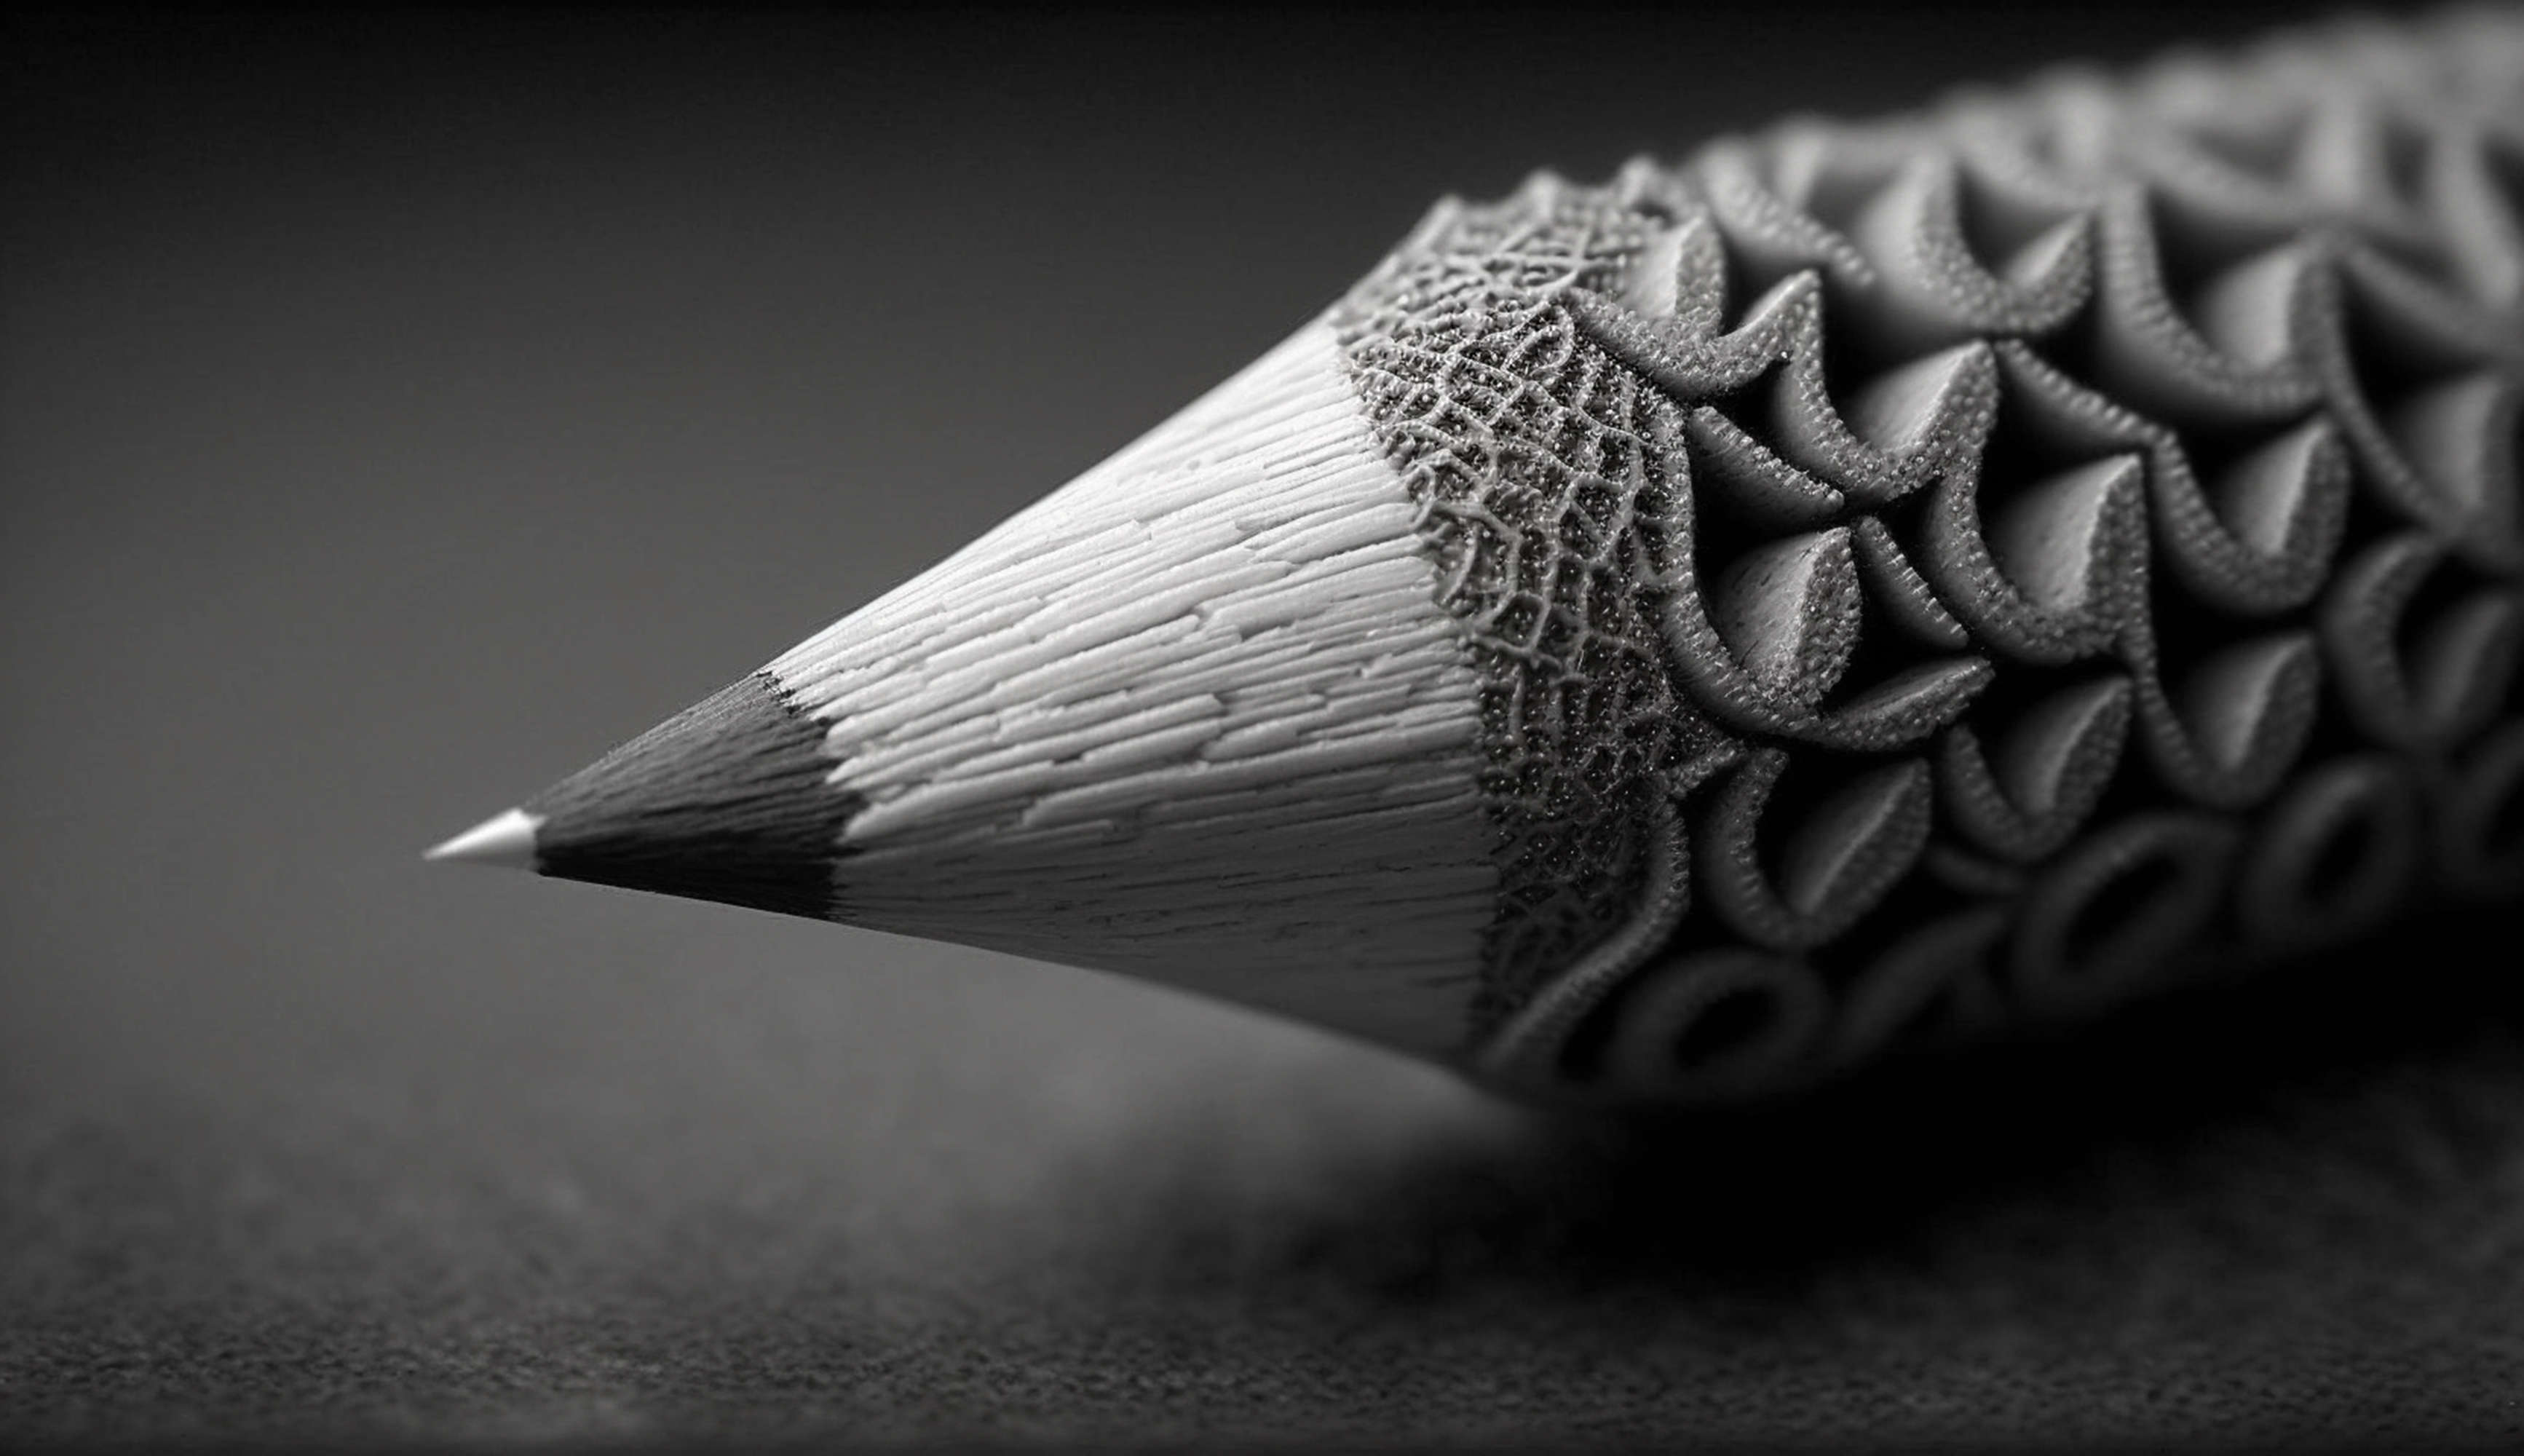
\includegraphics[width=\textwidth]{images/placeholder.png}
    \caption{Detailed Architecture -- Output and Recommendation Layer}
    \label{fig:arch3}
\end{figure}

%% =====================================================
\chapter{Project Objectives}
%% List specific, measurable goals. Each bullet should map to a deliverable.

\begin{itemize}
    \item To develop an intelligent system for automatic detection and classification using domain-specific data.

    \item To design and implement a scalable preprocessing and feature engineering pipeline.

    \item To build and evaluate a deep learning model achieving competitive performance on the selected dataset.

    \item To incorporate Explainable AI methods for transparent and interpretable predictions.

    \item To develop a recommendation module generating actionable insights using a retrieval-augmented generation approach.

    \item To create an interactive dashboard for visualizing predictions, explanations, and recommendations.

    \item To evaluate the system against baseline approaches using standard performance metrics.

    \item To build a modular and extensible framework suitable for future real-world deployment.
\end{itemize}

%% =====================================================
\chapter{Timeline using Gantt Chart}

\section{Timeline using Gantt Chart}

Figure~\ref{fig:gantt} illustrates the project timeline across the academic semester. The phases include literature review, dataset preprocessing, model development, explainability integration, recommendation engine development, and dashboard implementation.

\begin{figure}[H]
    \centering
    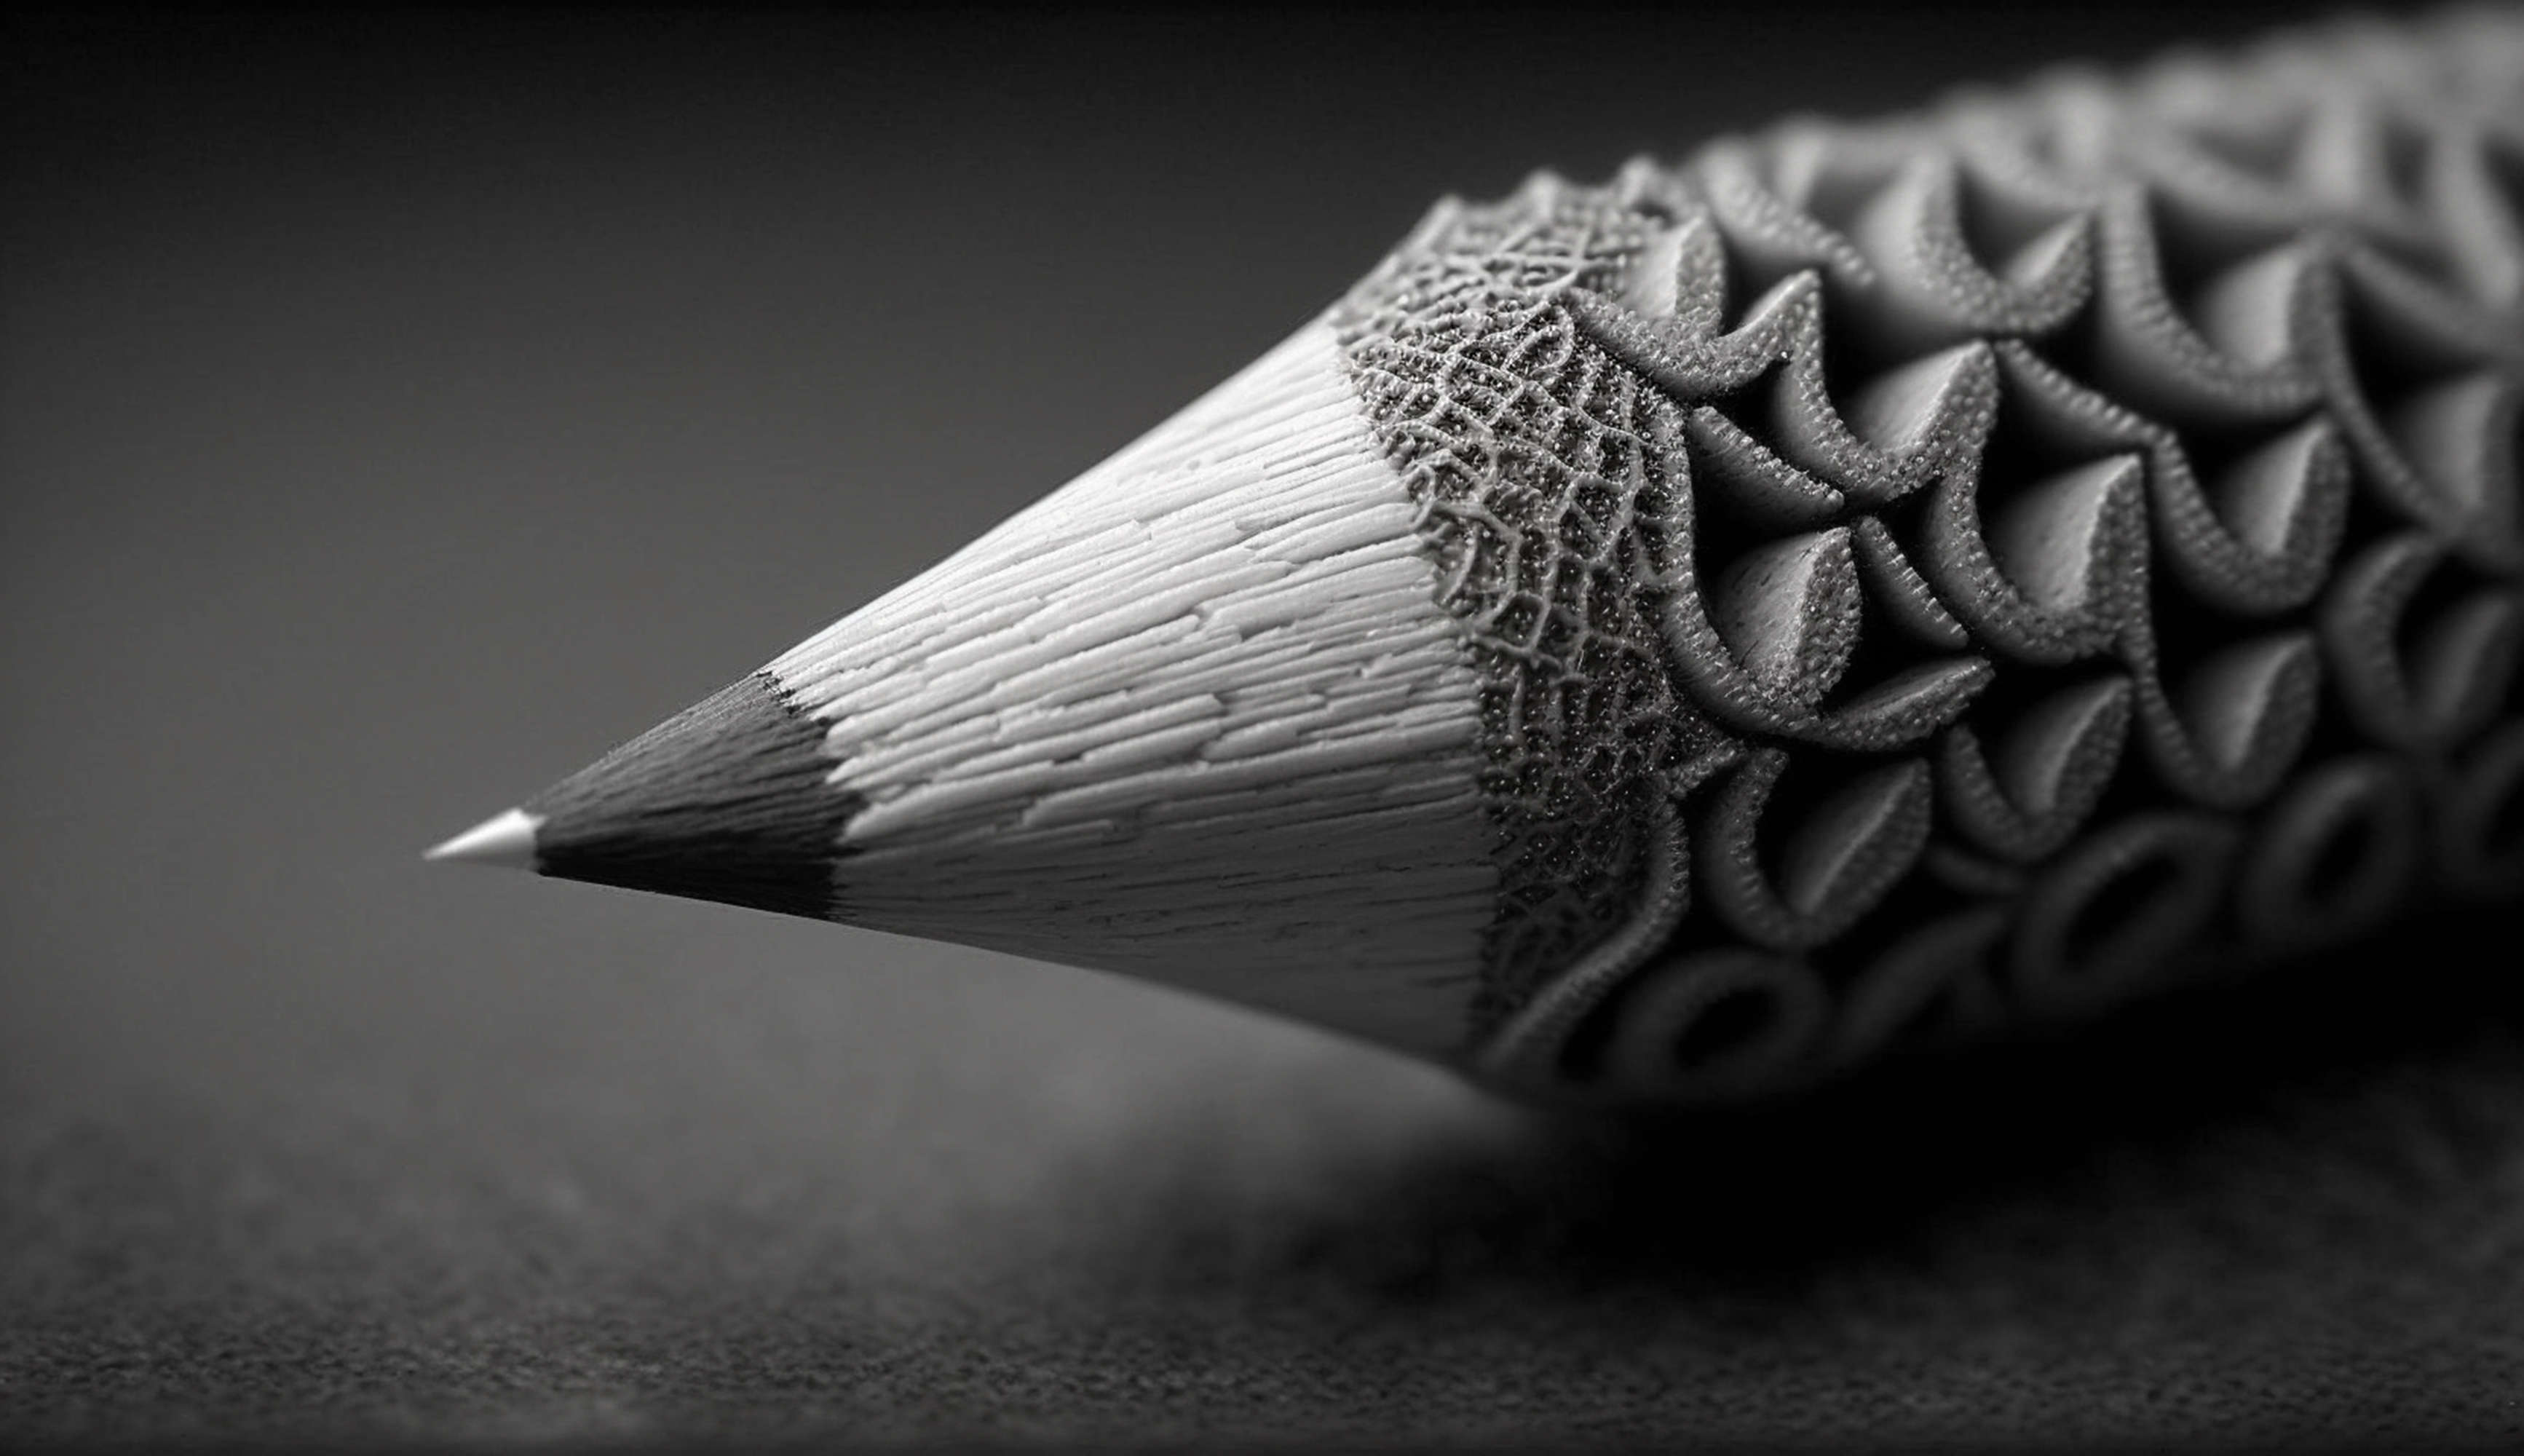
\includegraphics[width=\textwidth]{images/placeholder.png}
    \caption{Project Gantt Chart}
    \label{fig:gantt}
\end{figure}

%% =====================================================
\chapter{Hardware and Software Requirements}

\section{Hardware Requirements}

\begin{itemize}
    \item Personal Computer or Laptop (minimum 8 GB RAM)
    \item Intel i5 processor or higher
    \item Minimum 256 GB storage
    \item Internet connectivity
\end{itemize}

\section{Software Requirements}

\begin{itemize}
    \item Operating System: Windows / macOS / Linux
    \item Programming Language: Python 3.10 or higher
    \item Development Environment: Visual Studio Code / Jupyter Notebook
    \item Deep Learning Frameworks: TensorFlow or PyTorch
    \item Libraries: NumPy, Pandas, Scikit-learn, Matplotlib
    \item Explainable AI Tools: SHAP, LIME
    \item API Framework: FastAPI or Flask
    \item Vector Database: ChromaDB
    \item Version Control: Git and GitHub
\end{itemize}

%% =====================================================
\chapter{Sample Code}
%% Replace with a meaningful excerpt from your actual implementation.

\section{Sample Module Implementation}

The following snippet demonstrates a core component of the proposed system.

\begin{lstlisting}[language=Python, caption={Sample Preprocessing Utility}, label={code:sample}]
import numpy as np
import pandas as pd


def load_and_preprocess(filepath: str, target_col: str):
    """Load CSV and return normalized features and labels."""
    df = pd.read_csv(filepath).dropna()

    X = df.drop(columns=[target_col])
    y = df[target_col]

    numeric_cols = X.select_dtypes(include=[np.number]).columns
    X[numeric_cols] = (
        X[numeric_cols] - X[numeric_cols].mean()
    ) / X[numeric_cols].std()

    return X, y


if __name__ == "__main__":
    X, y = load_and_preprocess("data/sample.csv", target_col="label")
    print("Features:", X.shape)
    print("Labels:\n", y.value_counts())
\end{lstlisting}

%% =====================================================
\chapter{Project Demo Screenshots}
%% Replace each placeholder with your actual screenshot files.
%% Suggested location: images/screenshots/

Figure~\ref{fig:dashboard} shows the main dashboard of the proposed system.

\begin{figure}[H]
    \centering
    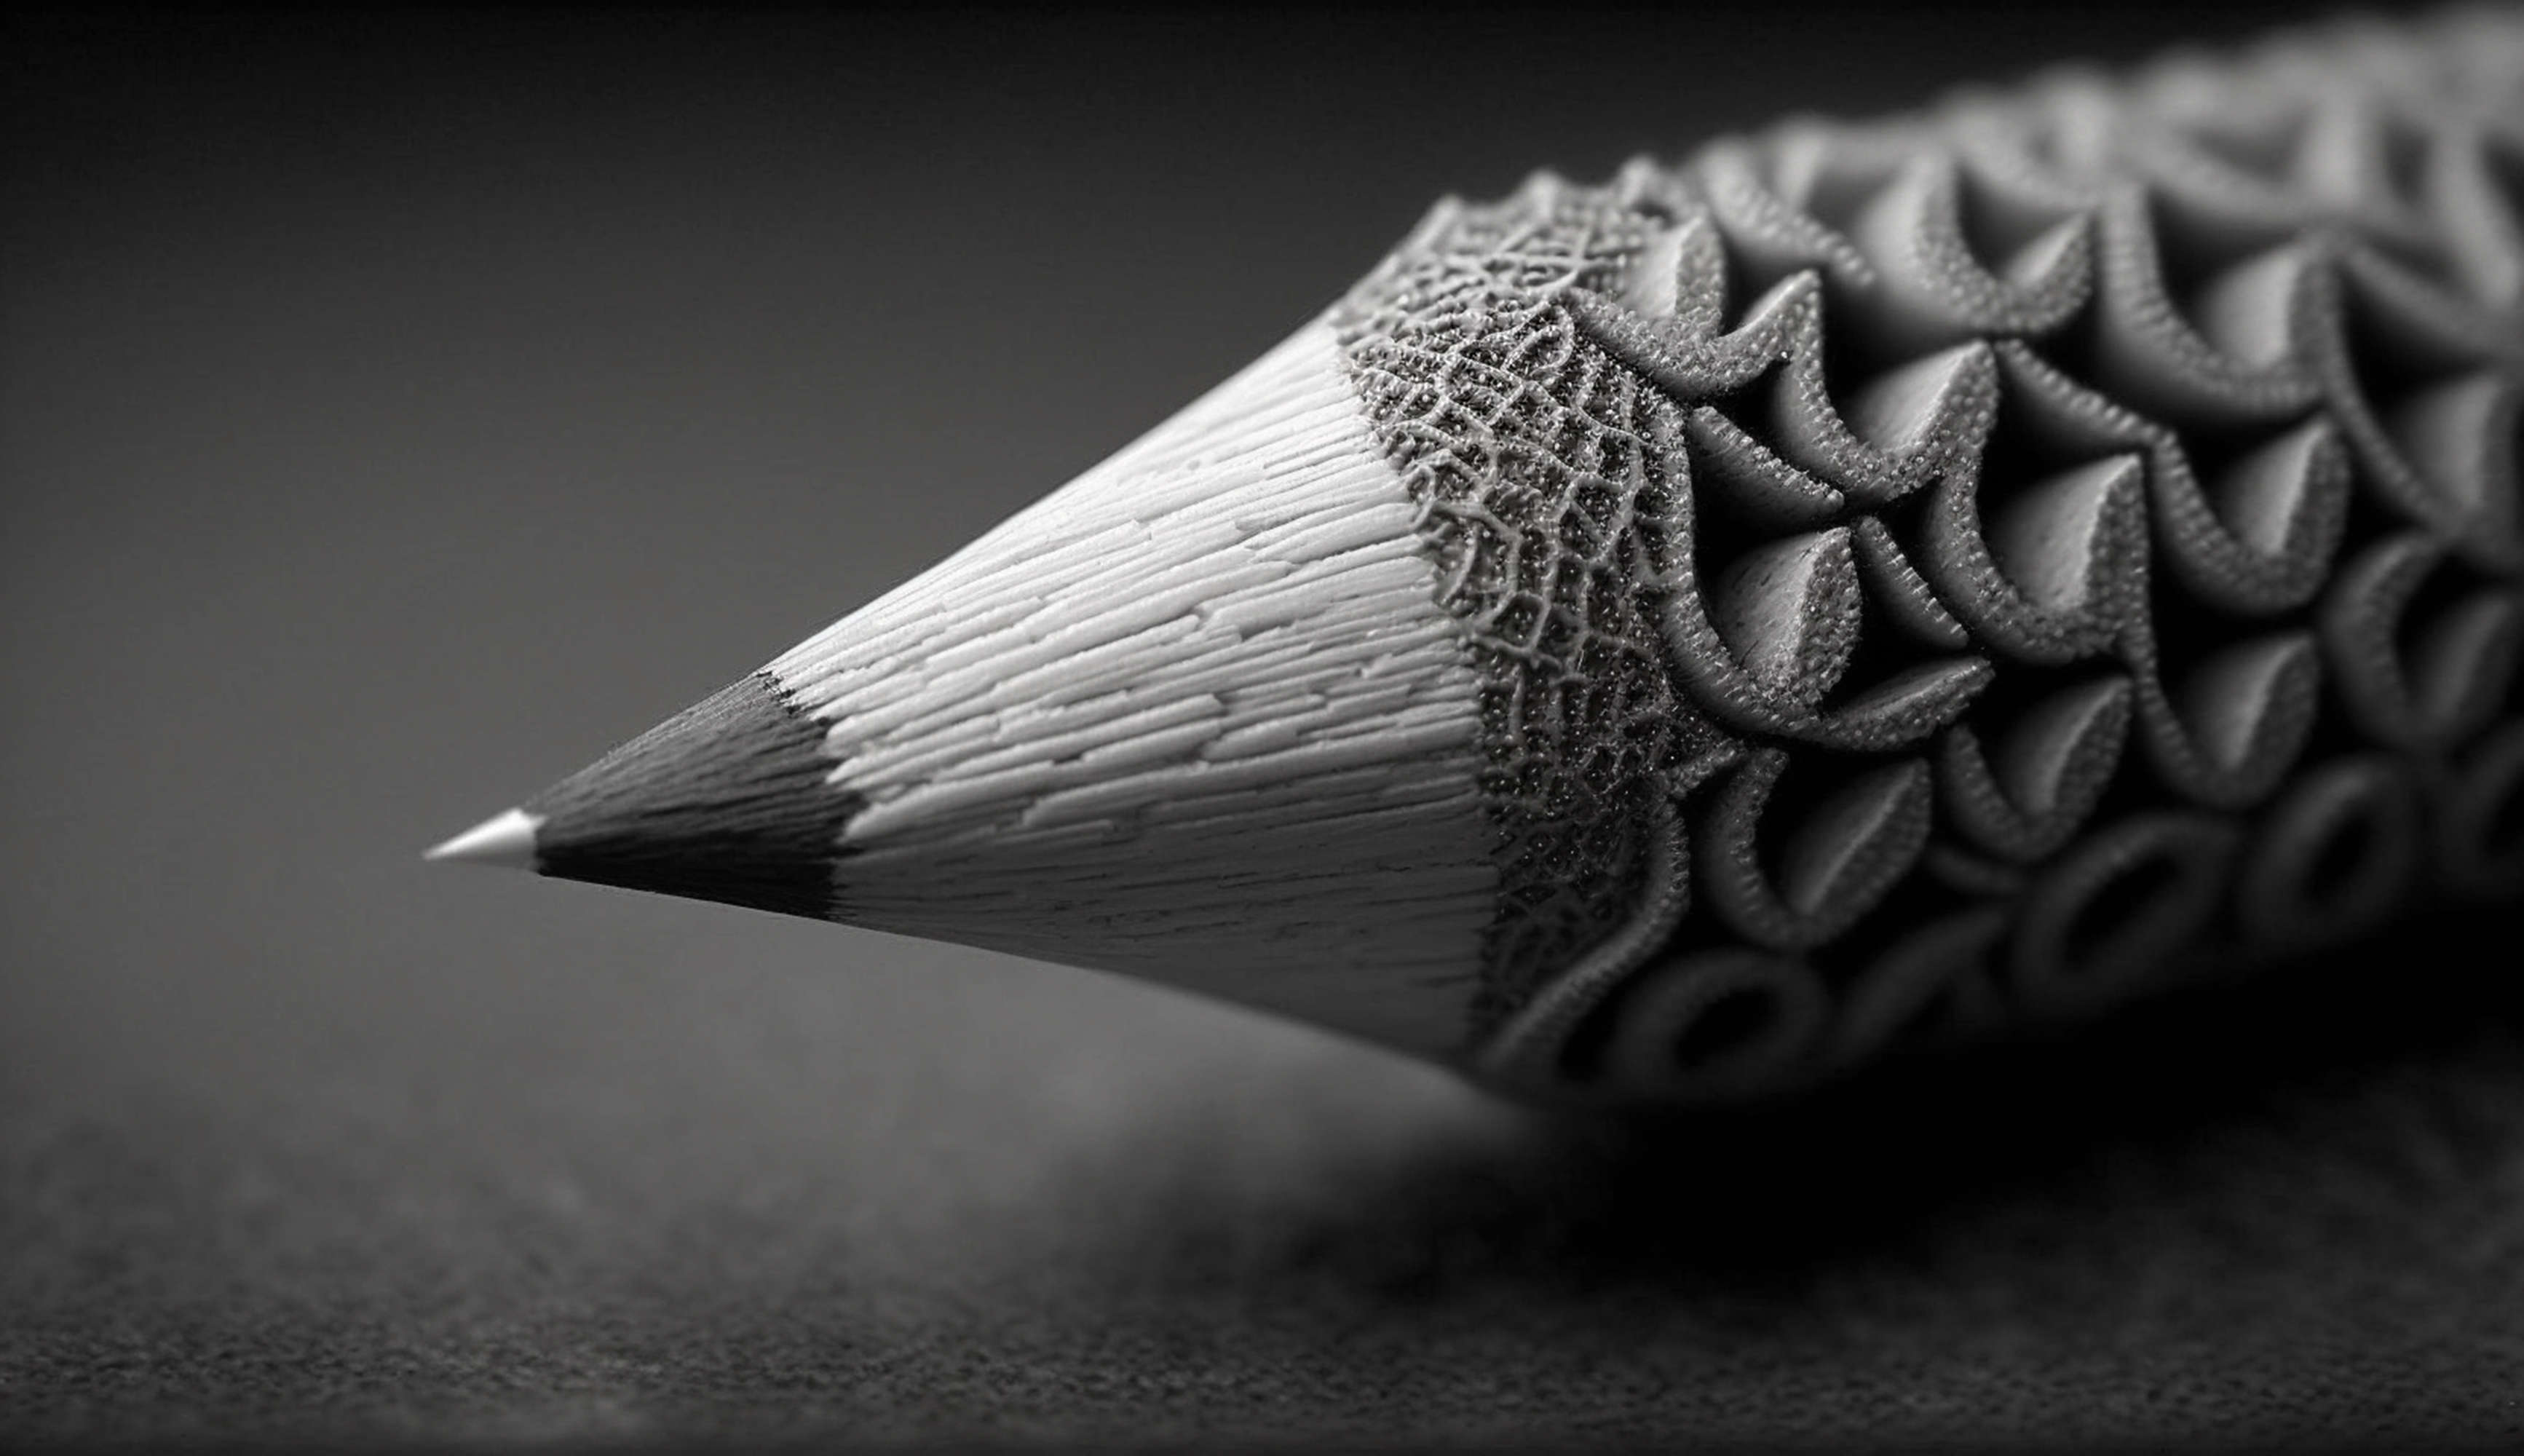
\includegraphics[width=\textwidth]{images/placeholder.png}
    \caption{Dashboard Interface of the Proposed System}
    \label{fig:dashboard}
\end{figure}

Figure~\ref{fig:feat_imp} shows the feature importance visualization from the explainability module.

\begin{figure}[H]
    \centering
    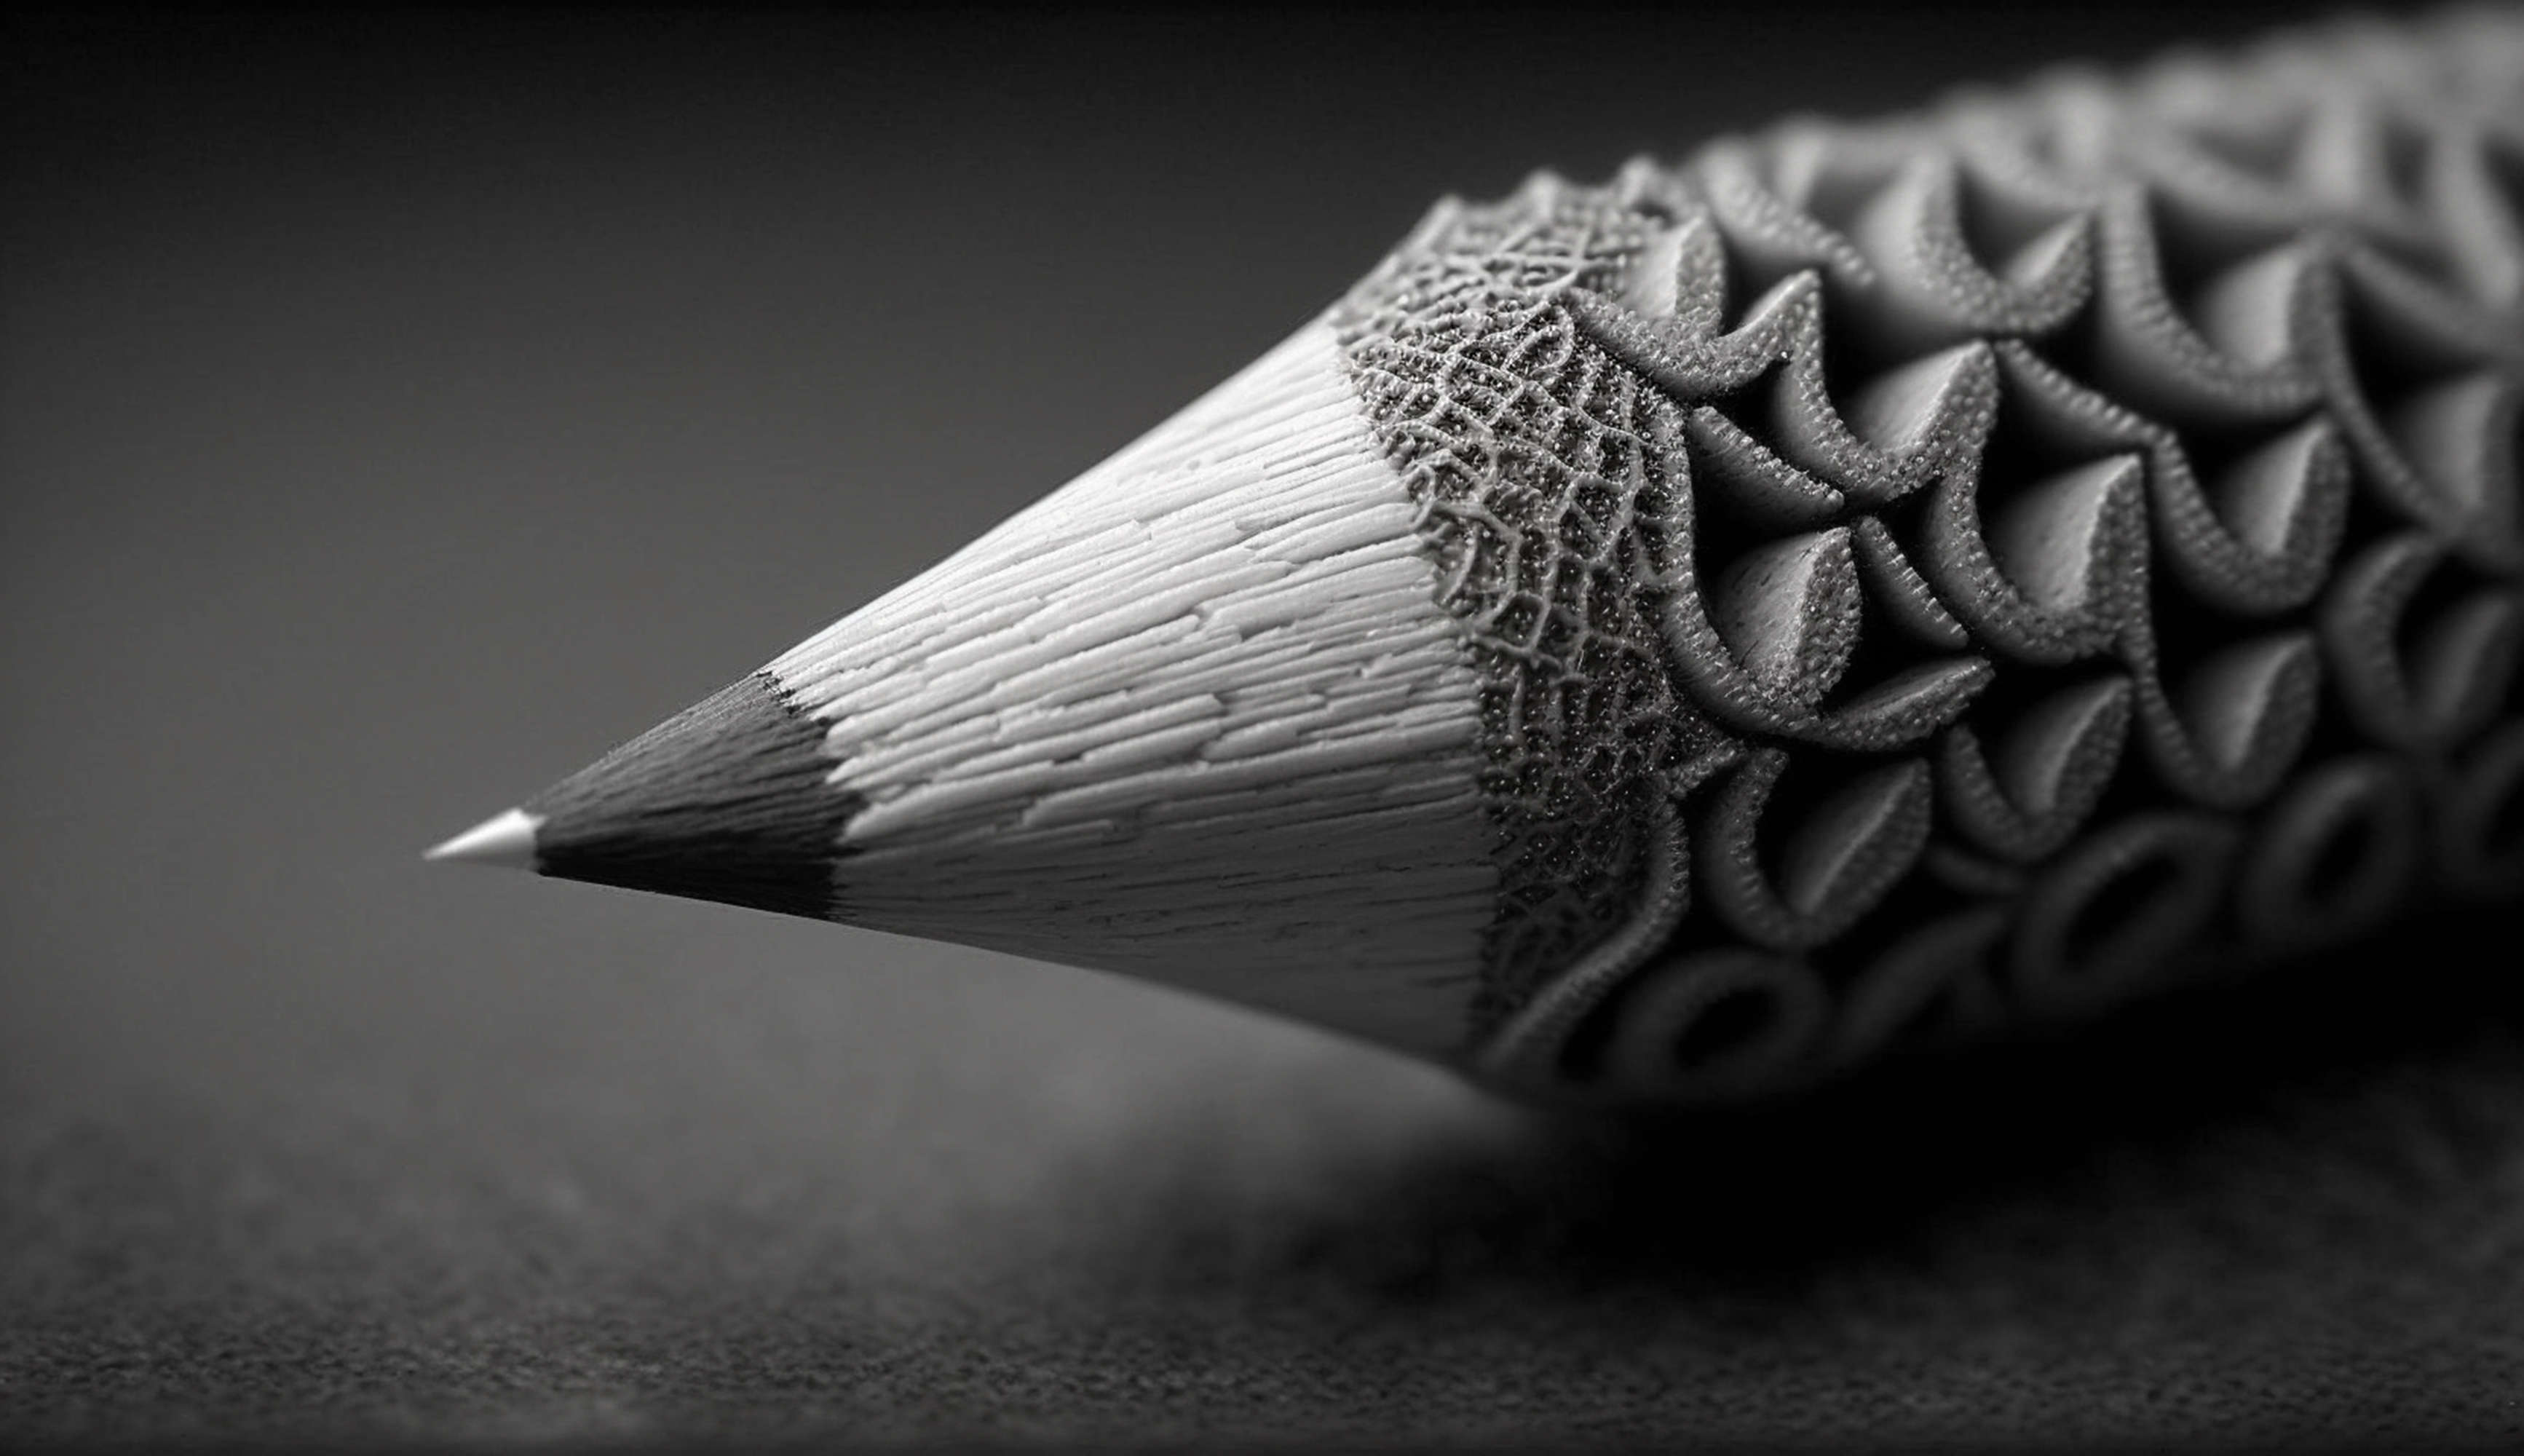
\includegraphics[width=0.9\textwidth]{images/placeholder.png}
    \caption{Feature Importance Visualization}
    \label{fig:feat_imp}
\end{figure}

Figure~\ref{fig:reco} shows the recommendations generated by the system.

\begin{figure}[H]
    \centering
    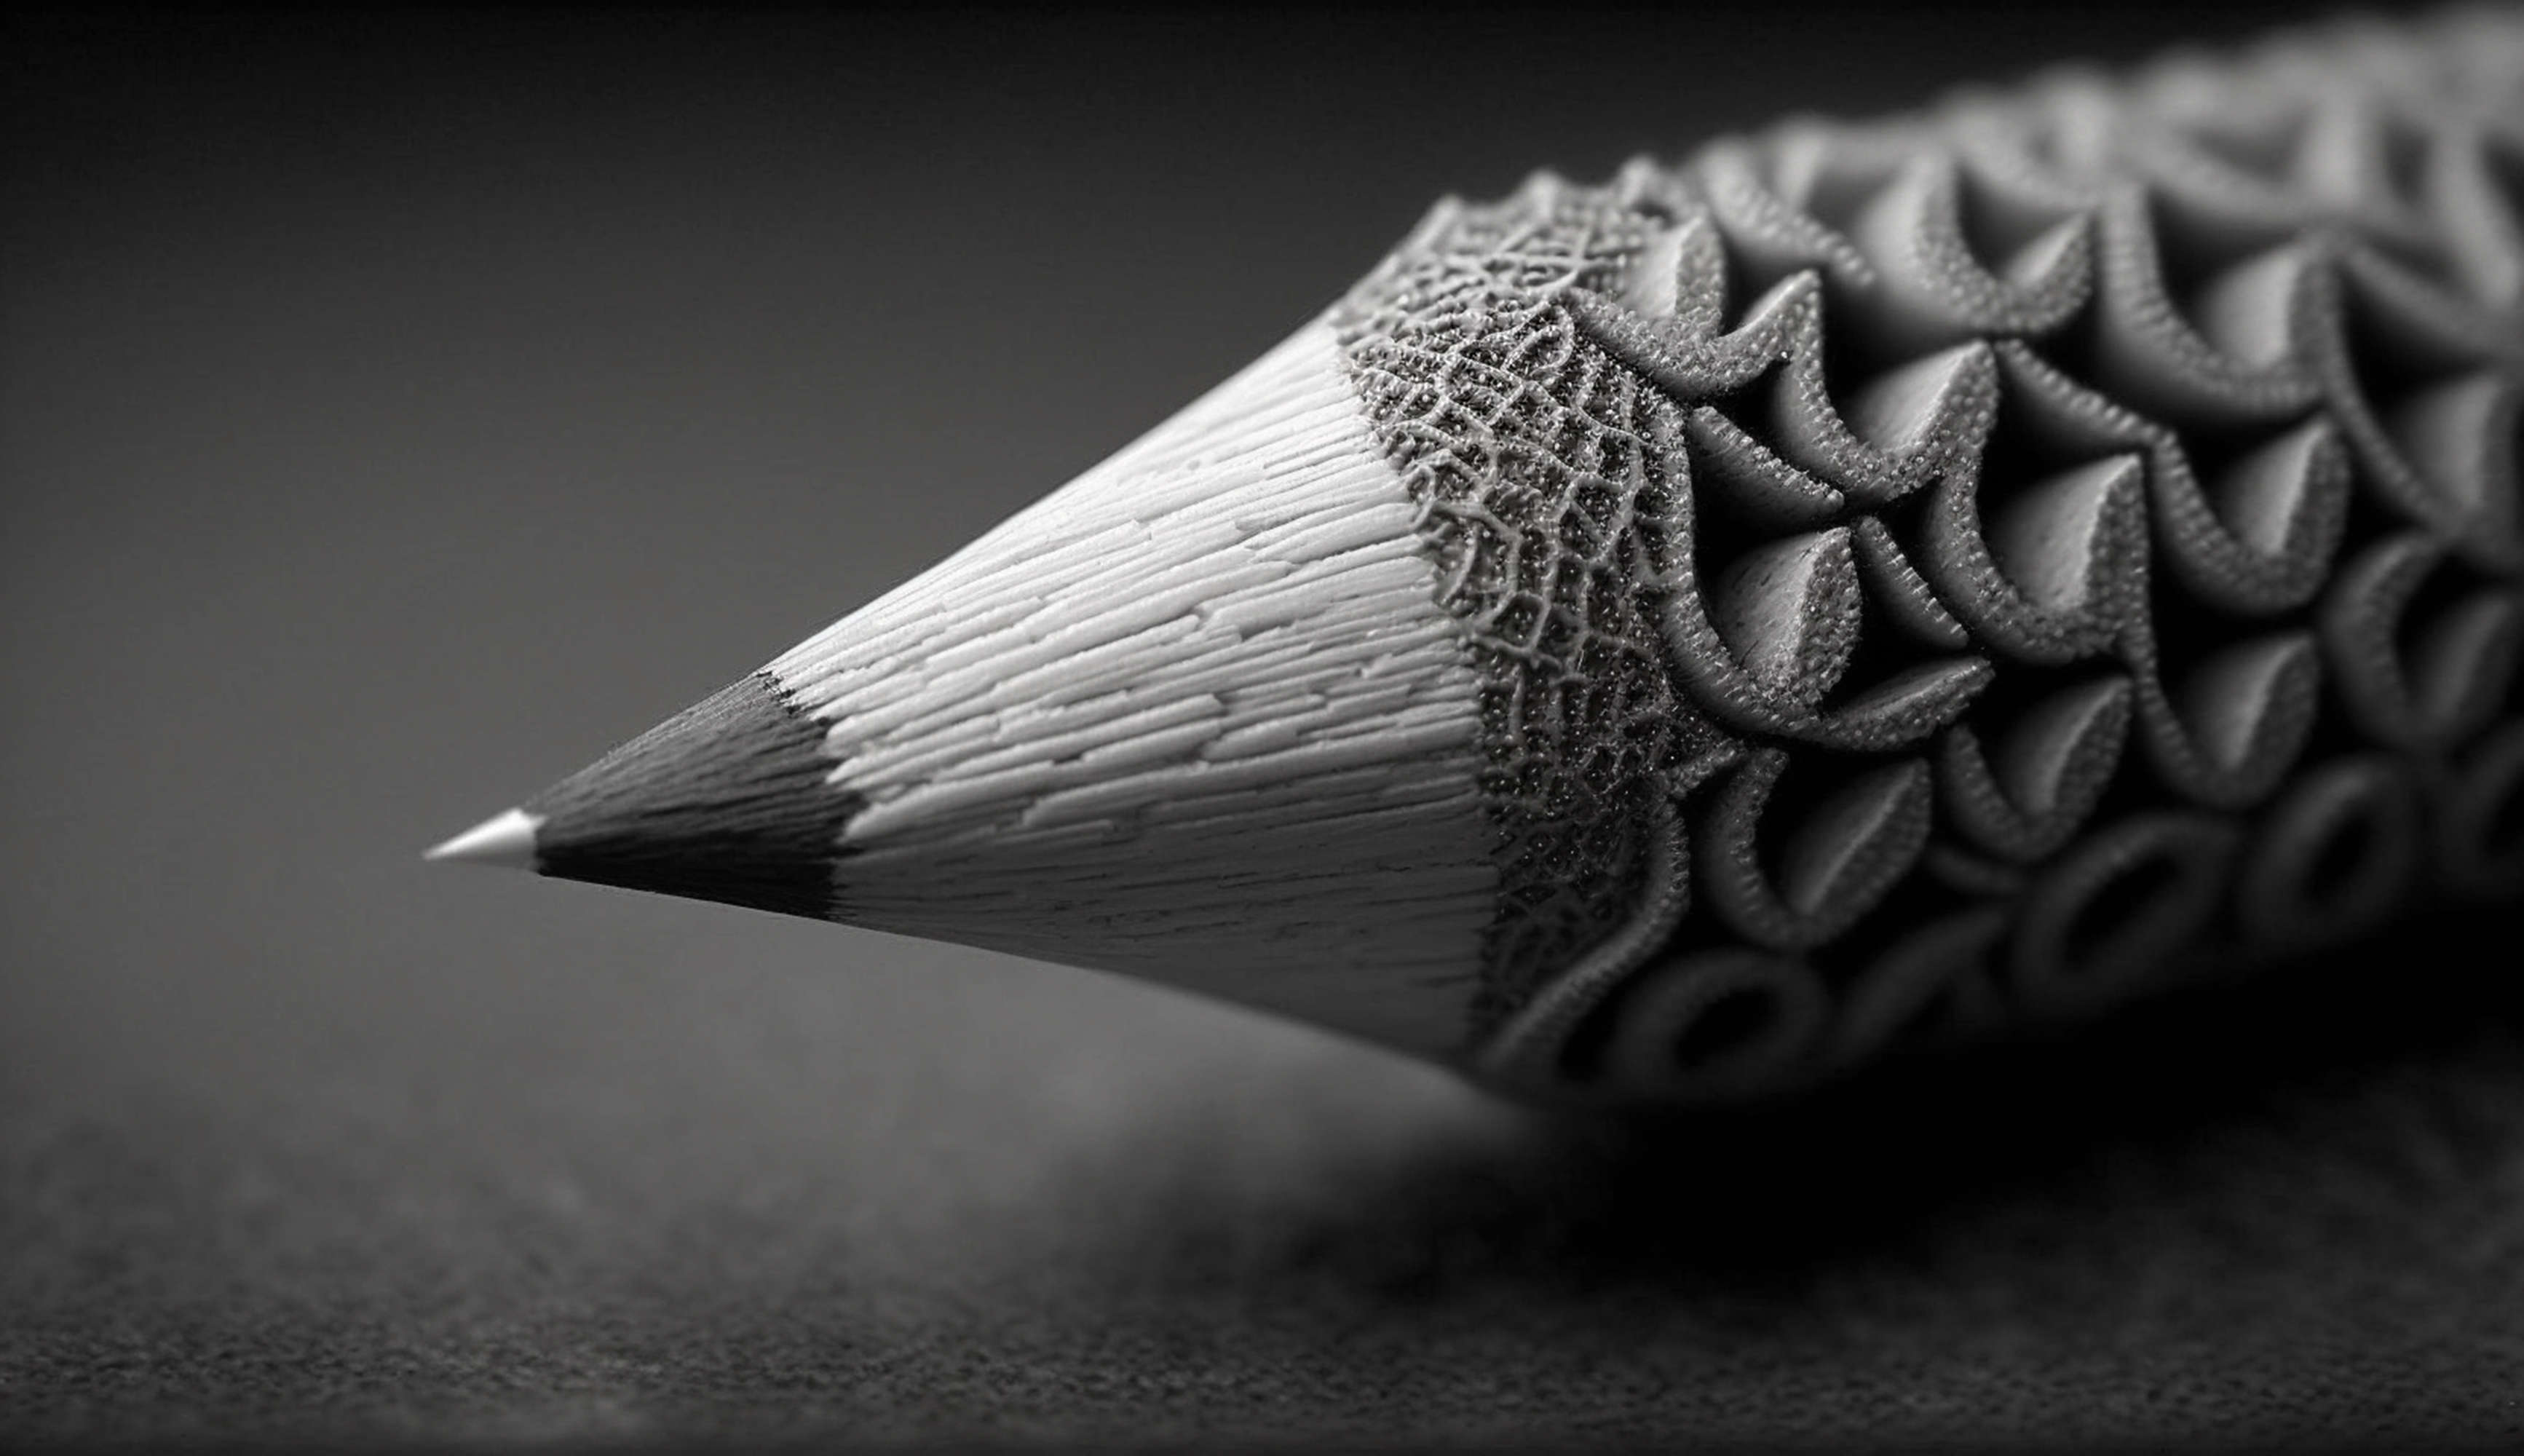
\includegraphics[width=\textwidth]{images/placeholder.png}
    \caption{System-Generated Recommendations}
    \label{fig:reco}
\end{figure}

%% =====================================================
\chapter{AI Tools Application}
%% List the AI tools your team used and what they were used for.

The proposed project utilized various AI-assisted development tools during research, design, implementation, and documentation.

\section{OpenAI -- ChatGPT}

\begin{itemize}
    \item Code generation for data preprocessing and model training
    \item Explaining deep learning and Explainable AI concepts
    \item Debugging machine learning pipelines
    \item Documentation and report writing support
\end{itemize}

\section{Google -- Gemini}

\begin{itemize}
    \item Research assistance and workflow planning
    \item Exploring multimodal learning and transformer architectures
    \item Architectural design and system workflow refinement
\end{itemize}

\section{GitHub -- GitHub Copilot}

\begin{itemize}
    \item Auto-completing repetitive code structures
    \item Writing model training and evaluation pipelines
    \item Debugging and improving code readability
\end{itemize}

%% =====================================================
\chapter{SDGs Met by Project with Proper Justification}
%% Select SDGs relevant to your project with specific justification.

\begin{itemize}
    \item \textbf{SDG 3: Good Health and Well-Being} ---
    The system supports health and well-being by enabling early detection and AI-driven decision support, providing personalized recommendations to improve user outcomes.

    \item \textbf{SDG 9: Industry, Innovation and Infrastructure} ---
    The project applies advanced AI technologies including deep learning and Explainable AI to build an innovative decision-support framework for intelligent automation.

    \item \textbf{SDG 4: Quality Education} ---
    The system and its documentation serve as a learning resource demonstrating practical integration of machine learning, explainability, and recommendation systems.

    \item \textbf{SDG 8: Decent Work and Economic Growth} ---
    By automating classification and decision-making tasks, the system reduces manual effort and supports more efficient, sustainable workflows.
\end{itemize}

%% =====================================================
\chapter{Purpose of the Project}

\section{Purpose of the Proposed System}

Lorem ipsum dolor sit amet, consectetur adipiscing elit. Sed do eiusmod tempor incididunt ut labore et dolore magna aliqua. The proposed system aims to develop an interpretable end-to-end AI framework combining machine learning, Explainable AI, and retrieval-augmented generation.

\section{Targeted Audience}

\begin{itemize}
    \item Domain experts who need to understand and validate AI predictions
    \item Researchers working on explainable AI and human-AI interaction
    \item Data scientists building production-grade ML pipelines
    \item Academic institutions using it as a reference implementation
\end{itemize}

\section{Expected Outcome of the Project}

\begin{itemize}
    \item Accurate multi-class classification on domain-specific data
    \item SHAP-based feature importance explanations per prediction
    \item Contextual recommendations via retrieval-augmented generation
    \item Interactive web dashboard presenting all outputs
\end{itemize}

\section{Research and Future Scope}

\begin{itemize}
    \item Integration with real-time data streams and edge devices
    \item Inclusion of additional data modalities
    \item Larger-scale real-world validation
    \item Mobile interface for end-user accessibility
\end{itemize}

%% =====================================================
\chapter{Research Paper and Plagiarism Report}

\section{Research Paper Details}

As part of the project work, a research paper titled
\textbf{``Your Full Research Paper Title Goes Here''}
has been prepared, covering the proposed system architecture, methodology,
experimental evaluation, and conclusion.

\section{Plagiarism and AI Detection Report}

The research paper was checked using Turnitin. The plagiarism and AI detection
reports are attached in the Appendix and confirm a low similarity index
satisfying originality requirements for academic submission.

%% =====================================================
\chapter{How to Use This Template}
%% Keep this chapter as-is when sharing with others.
%% It is a zero-knowledge cheat sheet for new users.

This chapter is a complete guide to using this template. No prior LaTeX knowledge is assumed.

%% ---
\section{Step 1 — Fill In Your Details}

Open \texttt{main.tex} and find the section at the top marked \textbf{FILL THIS}. Update every line in that block. Nothing else in the file needs to be touched for the title page, certificate, header, and acknowledgement to work correctly.

\begin{itemize}
    \item \texttt{\textbackslash ProjectTitle} --- Full title of your project
    \item \texttt{\textbackslash HeaderTitle} --- Short version used in the page header (keep it under 8 words)
    \item \texttt{\textbackslash AcademicYear} --- e.g.\ \texttt{2025--2026} (use two dashes for an en-dash)
    \item \texttt{\textbackslash StudentOne} through \texttt{\textbackslash StudentFour} --- Full names of all team members
    \item \texttt{\textbackslash USNOne} through \texttt{\textbackslash USNFour} --- Corresponding USNs
    \item \texttt{\textbackslash GuideName} --- Your guide's full name
    \item \texttt{\textbackslash GuideDesignation} --- Guide's designation and department
    \item \texttt{\textbackslash ProjectCoordinator} --- Project coordinator's name
    \item \texttt{\textbackslash HODName} --- Head of Department's full name
    \item \texttt{\textbackslash PrincipalName} --- Principal's full name
\end{itemize}

%% ---
\section{Step 2 — Compile Once to Check}

Before touching anything else, compile to confirm the template builds on your machine. Run these four commands in your terminal from inside the project folder:

\begin{lstlisting}[language=bash, caption={Full Compilation Sequence}]
pdflatex main.tex
bibtex main
pdflatex main.tex
pdflatex main.tex
\end{lstlisting}

You need to run \texttt{pdflatex} three times. The first pass builds the document and writes temporary files. \texttt{bibtex} processes the references. The second and third passes resolve cross-references and the table of contents. Skipping steps will cause \textbf{[?]} to appear instead of figure numbers or citations.

\textbf{Using an editor instead:} Overleaf, TeXstudio, and VS Code with the LaTeX Workshop extension all handle the multi-pass sequence automatically when you click Build. Overleaf is recommended if you have no LaTeX installation locally --- just upload the entire folder and compile.

%% ---
\section{Step 3 — Folder Structure}

Place your files according to the following layout:

\begin{itemize}
    \item \texttt{images/VTULogo.png} --- VTU logo (already included, do not rename)
    \item \texttt{images/DSCELogo.png} --- College logo (already included, do not rename)
    \item \texttt{images/placeholder.png} --- Used by all figures until you replace them. Copy any existing image and name it \texttt{placeholder.png} to keep compilation clean.
    \item \texttt{images/Diagrams/} --- Put all architecture diagrams, DFDs, and use case diagrams here
    \item \texttt{images/screenshots/} --- Put all dashboard and demo screenshots here
    \item \texttt{appendix/} --- Put your plagiarism and AI detection PDFs here
    \item \texttt{references.bib} --- All your references in BibTeX format
\end{itemize}

\textbf{Important:} File names are case-sensitive. \texttt{Dashboard.png} and \texttt{dashboard.png} are different files. Use lowercase names with underscores to avoid issues.

%% ---
\section{Step 4 — Adding Images}

Every figure in this template currently points to \texttt{images/placeholder.png}. Once you have your actual diagrams and screenshots ready, replace the path inside each \texttt{\textbackslash includegraphics} command with your real file path.

The full syntax for inserting an image is:

\begin{lstlisting}[language=TeX, caption={Image Block Syntax}]
\begin{figure}[H]
    \centering
    \includegraphics[width=0.75\textwidth]{images/Diagrams/your_image.png}
    \caption{Your caption text here}
    \label{fig:your_label}
\end{figure}
\end{lstlisting}

\textbf{Controlling image size} --- change the \texttt{width} value:

\begin{itemize}
    \item \texttt{width=\textbackslash textwidth} --- full page width (use for wide diagrams)
    \item \texttt{width=0.9\textbackslash textwidth} --- 90\% of page width
    \item \texttt{width=0.65\textbackslash textwidth} --- 65\% (good for portrait diagrams)
    \item \texttt{width=0.5\textbackslash textwidth} --- half width (good for small charts)
    \item \texttt{width=5cm} --- fixed size in centimetres
\end{itemize}

\textbf{Referring to a figure in text} --- use \texttt{\textbackslash ref\{fig:your\_label\}} and LaTeX will automatically insert the correct figure number:

\begin{lstlisting}[language=TeX, caption={Referring to a Figure}]
The architecture is shown in Figure~\ref{fig:your_label}.
\end{lstlisting}

%% ---
\section{Step 5 — Adding Lists}

\textbf{Bullet list} (unordered):

\begin{lstlisting}[language=TeX, caption={Bullet List}]
\begin{itemize}
    \item First point
    \item Second point
    \item Third point
\end{itemize}
\end{lstlisting}

\textbf{Numbered list} (ordered):

\begin{lstlisting}[language=TeX, caption={Numbered List}]
\begin{enumerate}
    \item First step
    \item Second step
    \item Third step
\end{enumerate}
\end{lstlisting}

Lists can be nested by placing one \texttt{itemize} or \texttt{enumerate} block inside another \texttt{\textbackslash item}.

%% ---
\section{Step 6 — Adding Code}

Use the \texttt{lstlisting} environment. Set \texttt{language} to \texttt{Python}, \texttt{bash}, \texttt{TeX}, \texttt{SQL}, \texttt{Java}, \texttt{C}, or \texttt{C++}.

\begin{lstlisting}[language=TeX, caption={Code Block Syntax}]
\begin{lstlisting}[language=Python, caption={Your caption}, label={code:your_label}]
# your code here
print("Hello")
\ end{lstlisting}
\end{lstlisting}

Note: remove the space between \texttt{\textbackslash} and \texttt{end} in actual use --- it is written that way here only to prevent the block from closing early.

%% ---
\section{Step 7 — Adding References}

Open \texttt{references.bib}. Each reference is one block called a BibTeX entry. The template already contains sample entries for every common type. Copy the one that matches your source and fill in the fields.

\textbf{Journal article:}
\begin{lstlisting}[language=TeX, caption={Journal Article BibTeX Entry}]
@article{yourkey2024,
  author  = {Surname, Firstname and Second, Author},
  title   = {Title of the Paper},
  journal = {Name of Journal},
  volume  = {12},
  number  = {3},
  pages   = {100--115},
  year    = {2024},
  doi     = {10.xxxx/xxxxxx}
}
\end{lstlisting}

\textbf{Conference paper:}
\begin{lstlisting}[language=TeX, caption={Conference Paper BibTeX Entry}]
@inproceedings{yourkey2023,
  author    = {Surname, Firstname and Co, Author},
  title     = {Title of the Paper},
  booktitle = {Proceedings of the Conference Name},
  pages     = {45--52},
  year      = {2023},
  doi       = {10.1109/xxxxxx}
}
\end{lstlisting}

\textbf{Website or dataset:}
\begin{lstlisting}[language=TeX, caption={Website or Dataset BibTeX Entry}]
@misc{yourkey2022,
  author       = {Author, Name},
  title        = {Title of the Resource},
  year         = {2022},
  howpublished = {\url{https://example.com}},
  note         = {Accessed: January 2024}
}
\end{lstlisting}

The key (e.g.\ \texttt{yourkey2024}) is what you use to cite the reference in text:

\begin{lstlisting}[language=TeX, caption={Citing a Reference}]
According to Smith et al.~\cite{yourkey2024}, ...
\end{lstlisting}

The \texttt{\textasciitilde} before \texttt{\textbackslash cite} adds a non-breaking space so the citation number never wraps onto a new line by itself.

%% ---
\section{Step 8 — Adding More PDFs to the Appendix}

To attach an additional PDF (e.g.\ your actual research paper), add the following block inside the Appendix chapter at the bottom of \texttt{main.tex}:

\begin{lstlisting}[language=TeX, caption={Attaching a PDF to the Appendix}]
\section{Your Section Title}

Brief description of what this document is.

\includepdf[
    pages=-,
    pagecommand={\thispagestyle{mainstyle}}
]{appendix/your_file.pdf}
\end{lstlisting}

\texttt{pages=-} means include all pages. To include only specific pages, use \texttt{pages=\{1,3,5\}} or a range like \texttt{pages=\{2-4\}}.

%% ---
\section{Quick Reference Card}

\begin{itemize}
    \item \textbf{Bold text:} \texttt{\textbackslash textbf\{your text\}}
    \item \textbf{Italic text:} \texttt{\textbackslash textit\{your text\}}
    \item \textbf{Inline code / filenames:} \texttt{\textbackslash texttt\{your text\}}
    \item \textbf{New section:} \texttt{\textbackslash section\{Section Title\}}
    \item \textbf{New subsection:} \texttt{\textbackslash subsection\{Subsection Title\}}
    \item \textbf{Line break in title page:} \texttt{\textbackslash\textbackslash}
    \item \textbf{En-dash (year range):} \texttt{2025\texttt{-{}-}2026} renders as 2025--2026
    \item \textbf{Non-breaking space:} \texttt{\textasciitilde} (use before \texttt{\textbackslash cite} and \texttt{\textbackslash ref})
    \item \textbf{Percentage sign:} \texttt{\textbackslash\%} (plain \% starts a comment)
    \item \textbf{Ampersand:} \texttt{\textbackslash\&}
    \item \textbf{Comment (ignored by compiler):} start the line with \texttt{\%\%}
\end{itemize}

%% =====================================================

\renewcommand{\bibname}{References and Bibliography}
\addcontentsline{toc}{chapter}{References and Bibliography}
\bibliographystyle{unsrt}
\bibliography{references}

\clearpage
\appendix
\pagestyle{mainstyle}

\chapter{Research Paper, Plagiarism and AI Detection Reports}

%% -------------------------------------------------------
%% TEMPLATE NOTE:
%% The PDFs attached below are sample files included only
%% to keep the template compiling cleanly out of the box.
%% Replace them with your actual reports before submission:
%%
%%   appendix/sample_IEEE_doc.pdf  ->  your research paper / plagiarism report
%%   appendix/sample.pdf           ->  your AI detection report
%%
%% Rename the files if needed and update the paths below.
%% -------------------------------------------------------

\section{Turnitin Similarity Report}

The Turnitin similarity report begins from the next page.


\includepdf[
    pages=-,
    pagecommand={\thispagestyle{mainstyle}}
]{appendix/sample_IEEE_doc.pdf}

\section{Turnitin AI Detection Report}

The Turnitin AI detection report begins from the next page.

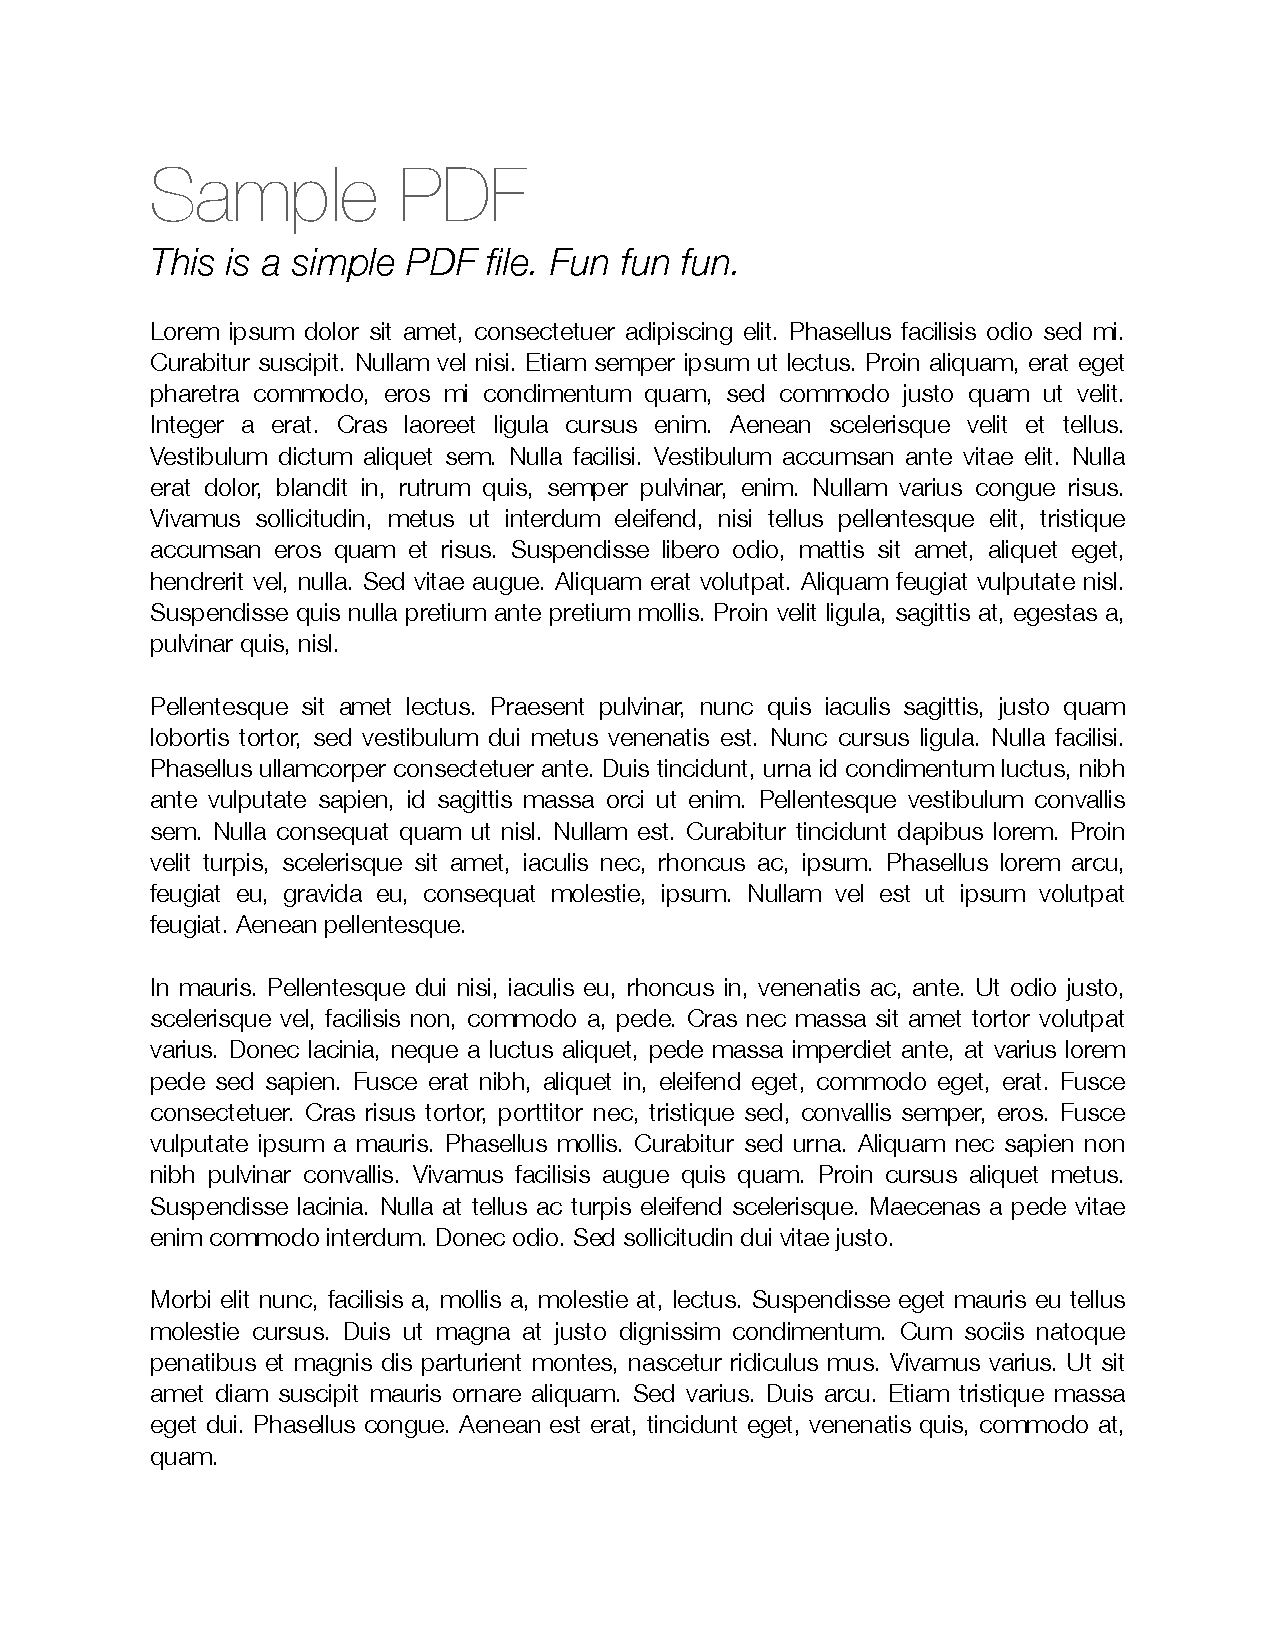
\includepdf[
    pages=-,
    pagecommand={\thispagestyle{mainstyle}}
]{appendix/sample.pdf}

\end{document}